\documentclass[12pt]{article}
\usepackage[T2A]{fontenc}
\usepackage[utf8]{inputenc}
\usepackage[russian, english]{babel}
\usepackage{amsmath}
\usepackage{amssymb}
\usepackage{amsthm}
\usepackage{amsfonts}
\usepackage[usenames]{color}
\usepackage{tikz}
\usepackage{comment}
\usepackage{hyperref}
\usepackage{blindtext}
\usepackage{centernot}
\usepackage{geometry}
 \geometry{
 a4paper,
 total={170mm,257mm},
 left=20mm,
 top=20mm,
 }


\title{Тропическая линейная алгебра}
\author{Никита Шапошник, Б05-024\\ научный руководитель: А. Э. Гутерман}

\newtheorem{theorem}{Теорема}[section]
\newtheorem{definition}[theorem]{Определение}
\newtheorem{proposition}[theorem]{Утверждение}
\newtheorem{remark}[theorem]{Замечание}
\newtheorem{lemma}[theorem]{Лемма}
\newtheorem{corollary}[theorem]{Следствие}
\newtheorem{algorithm}[theorem]{Алгоритм}

\date{}

\begin{document}
\maketitle
\section{Введение}
Тропическая математика была придумана бразильским математиком Имре Саймоном (Imre Simon, \cite{ImreSimon}) в конце XX века (название произошло от его места жительства). Матрицы над тропическим полукольцом имеют приложения в теории графов, отпимизации и биологии. В настоящей работе мы будем рассматривать матрицы над тропическим полукольцом, их связь с графами и некоторые их индексы: экспоненту, скрамблинг индекс, индекс цикличности и границы $T$.

\section{Определения}
\begin{definition}
Тропическая алгебра (\cite{glanceOnTropicalLA},
        \cite{tropicalMath}) --- это множество $\mathbb{R}_{\max} = \mathbb{R} \cup \{ -\infty\}$ с операциями сложения $\oplus$ и умножения $\odot$: \begin{align*}
            a \oplus b &= \max(a, b)\\
            a \odot b &= a + b
        \end{align*}      
        или множество $\mathbb{R}_{min} = \mathbb{R} \; \cup \; \{ \infty\}$ с другой операцией сложения и идентичным умножением: \begin{align*}
            a \oplus b &= min(a, b)\\
            a \odot b &= a + b.
        \end{align*}
\end{definition}

В дальнейшем мы будем работать с $\mathbb{R}_{\max}$.

\begin{lemma} [Свойства тропической алгебры, см. \cite{glanceOnTropicalLA}, \cite{tropicalMath}, \cite{Volchenko}] Тропическая алгебра обладает следующими свойствами: для любых $a, b, c \in \mathbb{R}_{\max}$ верно:
\begin{itemize}
	\item Сложение и умножение ассоциативны.
	\item Сложение и умножение коммутативны.
	\item Дистрибутивность: $a \odot (b \oplus c) = a \odot b \oplus a \odot c$.
	\item $-\infty$ --- нулевой элемент: $a \odot -\infty = a$.
	\item $0$ --- единичный элемент: $a \oplus 0= a$.
	\item Результат умножения на тропический ноль --- это тропический ноль: $a \odot -\infty = -\infty$.
	\item Несуществование обратного по сложению: если $a \neq -\infty$, \\то $a \oplus b \ge a > -\infty$.
\end{itemize}
\end{lemma}
\begin{corollary}
Тропическая алгебра является полукольцом.
\end{corollary}
\begin{definition}
Граф (в рамках данной задачи) ${\mathcal{G}(V,E)}$ --- совокупность двух множеств – непустого множества $V = V(\mathcal{G})$ и множества $E = E(\mathcal{G}) \subseteq V^2$. Множество ${V}$ называется множеством вершин, множество ${E}$ называется множеством рёбер.

Если для любого ребра $(u, v) \in E(\mathcal{G})$ верно, что обратное ребро $(v, u) \in E(\mathcal{G})$ --- тоже лежит в графе, то граф $\mathcal{G}$ называется неориентированным, в противном случае --- ориентированным.

Путем из вершины $u$ в вершину $v$ в графе $\mathcal{G}$ называется последовательность вершин $u, w_1, w_2, \dots, w_l, v \in V(\mathcal{G})$ и последовательность ребер $(u, w_1), (w_1, w_2), \dots, (w_l, v) \in E(\mathcal{G})$, где вершины и ребра могут повторяться. Путь называется простым, если вершины в нём не повторяются. Длиной пути называется количество ребер в нем. Обозначим через $\mathcal{W}^t(i \rightarrow j)$ множество всех путей из вершины $i$ в вершину $j$ длины $t$, а через $\mathcal{W}(i \rightarrow j)$ --- множество всех путей из вершины $i$ в вершину $j$.

Граф $\mathcal{G}(V, E)$ со введенной функцией $P : E \rightarrow \mathbb{R}$ называется взвешенным графом. Весом пути называется тропическое произведение (т.е. вещественная сумма) весов всех ребер в пути. Обозначим вес пути $W$ через $p(W)$. 

Ориентированный граф называется сильно связным, если для любых $u, v \in V(\mathcal{G})$ существует путь из $u$ в $v$ и из $v$ в $u$.
        
Граф $\mathcal{G}'$ называется подграфом графа $\mathcal{G}$, если $\mathcal{G}'$ получен из $\mathcal{G}$ удалением некоторых ребер и, возможно, вершин. Иначе, $V(\mathcal{G}') \subseteq V(\mathcal{G})$ и\\ $E(\mathcal{G}') \subseteq E(\mathcal{G})$.

Обхватом графа $\mathcal{G}$ называется наименьшая длина цикла в $\mathcal{G}$ и обозначается как $g(\mathcal{G})$. Через $\hat{g}(\mathcal{G})$ обозначается максимальный обхват среди всех компонент сильной связности графа $\mathcal{G}$.

Граф $\mathcal{H}(U, F)$ называется индуцированным подграфом графа $\mathcal{G}(V, E)$, порожденным под-\\множеством вершин $U \subset V$, если ребрами $\mathcal{H}$ являются те и только те ребра множества $E$, оба конца которых принадлежат $U$.
\end{definition}

\section{Примитивность вещественной неотрицательной матрицы}
\begin{definition}
Вещественная матрица $A$ называется примитивной, если существует натуральное число $m$ такое, что $A^m$ положительна, то есть все числа в ней положительны. При этом наименьшее такое $m$ называется экспонентой матрицы и обозначается через $exp(A)$.
\end{definition}

\begin{theorem}[Критерий примитивности матрицы, см.\cite{Brualdi}]
 Неотрицательная квадратная матрица порядка $n$ над $\mathbb{R}$ примитивна тогда и только тогда, когда граф смежности этой матрицы сильно связен и НОК всех длин замкнутых путей (циклов) равно 1.
\end{theorem}
\begin{theorem}[Виландта, {\cite{wielandt}}]
Если неотрицательная квадратная матрица порядка $n$ над полем вещественных чисел примитивна, то ее экспонента не превосходит число Виландта $Wi(n) = n^2-2n+2$.
\end{theorem}

\section{Примитивность тропических матриц}
\begin{remark}
Примитивность и экспонента тропической матрицы определяется так же, как и в вещественном случае, с отличием лишь в том, что в степени матрицы не должно быть нулей тропичeского полукольца, т.е. $-\infty$.
\end{remark}

\subsection{Матрицы $2\times2$}
\begin{proposition}
Матрица $A = \begin{pmatrix}
a & b \\
c & d
\end{pmatrix}$ над тропическим полукольцом примитивна тогда и только тогда, когда $b \neq -\infty \wedge c \neq -\infty \wedge (a \neq -\infty \vee d \neq -\infty)$; причем ее экспонента равна 2.
\end{proposition}
\begin{proof}[\textbf{Доказательство}]
Если перемножить матрицы, у которых в правом верхнем углу стоят $-\infty$, то у результата будет стоять $-\infty$ в том же углу:
\begin{multline*}
\begin{pmatrix}
a & -\infty \\
c & d
\end{pmatrix} \cdot \begin{pmatrix}
a' & -\infty \\
c' & d'
\end{pmatrix} = \begin{pmatrix}
\dots & a \odot -\infty \oplus -\infty \odot d' \\
\dots & \dots
\end{pmatrix} = \begin{pmatrix}
\dots & -\infty \\
\dots & \dots
\end{pmatrix}
\end{multline*}
Аналогично с левым нижнем углом. Значит, в правом верхнем и в левом нижним углах не могут стоять $-\infty$.

Перемножим 2 матрицы, у которых на главной диагонали стоят $-\infty$:
\begin{multline*}
\begin{pmatrix}
-\infty & b \\
c & -\infty
\end{pmatrix} \cdot \begin{pmatrix}
-\infty & b' \\
c' & -\infty
\end{pmatrix} = \\ = \begin{pmatrix}
... & 
-\infty \odot b' \oplus b \odot -\infty \\
c \odot -\infty \oplus -\infty \odot c' &
...
\end{pmatrix} = \begin{pmatrix}
\dots & -\infty \\
-\infty & \dots
\end{pmatrix}
\end{multline*}
У результата стоят $\infty$ на побочной диагонали. Перемножим такую матрицу с матрицей с $\infty$ на главной диагонали:
\begin{multline*}
\begin{pmatrix}
a & -\infty \\
-\infty & d
\end{pmatrix} \cdot \begin{pmatrix}
-\infty & b \\
c & -\infty
\end{pmatrix} = \\ = \begin{pmatrix}
a \odot -\infty \oplus -\infty \odot c & 
... \\
... & 
-\infty \odot b \oplus -\infty \odot d
\end{pmatrix} = \begin{pmatrix}
-\infty & \dots \\
\dots & -\infty
\end{pmatrix}
\end{multline*}
Снова получилась матрица с $-\infty$ на главной диагонали. Значит, в любой степени матрицы с $-\infty$ на главной диагонали будут $-\infty$. Значит, она не может быть примитивной.

Проверим, что матрица с описанными выше ограничениями будет примитивной:
\begin{equation*}A^{\odot 2} = \begin{pmatrix}
a & b \\
c & d
\end{pmatrix}^{\odot 2} = \begin{pmatrix}
a \odot a \oplus b \odot c & a \odot b \oplus b \odot d \\
a \odot c \oplus c \odot d & b \odot c \oplus d \odot d
\end{pmatrix} = \begin{pmatrix}
\max(2a, b + c) & b + \max(a, d) \\
c + \max(a, d) & \max(b + c, 2d)
\end{pmatrix}
\end{equation*}
Равным $-\infty$ в этой матрице может быть или $a$, или $d$, или никто из них. В любом случае, в квадрате не будет $-\infty$. Значит, $A$ является примитивной с показателем степени 2.
\end{proof}
\subsection{Обобщение теоремы Виландта на тропические матрицы}
\begin{definition}
$\mathbb{B} = \{\textbf{0,1}\}$ --- множество с сложением, аналогичным дизъюнкции, и умножением, аналогичным конъюнкции:
\begin{center}
\begin{tabular}{|c|c|c|}
\hline
$+$ & $\textbf{0}$ & $\textbf{1}$ \\
\hline
$\textbf{0}$ & $\textbf{0}$ & $\textbf{1}$ \\
\hline
$\textbf{1}$ & $\textbf{1}$ & $\textbf{1}$ \\
\hline
\end{tabular}
\quad
\begin{tabular}{|c|c|c|}
\hline
$\cdot$ & $\textbf{0}$ & $\textbf{1}$ \\
\hline
$\textbf{0}$ & $\textbf{0}$ & $\textbf{0}$ \\
\hline
$\textbf{1}$ & $\textbf{0}$ & $\textbf{1}$ \\
\hline
\end{tabular}
\end{center}
\end{definition}
\begin{remark}
Примитивность и экспонента матрицы над $\mathbb{B}$ определяется так же, как и в вещественном случае.
\end{remark}

\begin{theorem}[Виландта для матриц над $\mathbb{B}$]
Если матрица $A \in M_n(\mathbb{B})$ примитивна, то ее экспонента не превосходит $n^2-2n+2$.
\end{theorem}
\begin{proof}[\textbf{Доказательство}]
Рассмотрим функцию $\beta' : \mathbb{R}_{\geq0} \rightarrow \mathbb{B}$ такую, что
\begin{equation}
    \beta'(t) = 
    \begin{cases}
        \textbf{1}, t \neq 0 \\
        \textbf{0}, t = 0
    \end{cases}
\end{equation}
и функцию $B' : M_n(\mathbb{R}_{\geq0}) \rightarrow M_n(\mathbb{B})$, действующая функцией $\beta'$ поэлементно:
\begin{equation}
    B' : A=(a_{ij}) \mapsto B'(A)=(\beta'(a_{ij}))
\end{equation}
\begin{lemma} \label{l:B'}
$B'$ --- гомоморфизм.
\end{lemma}
\begin{proof}[\textbf{Доказательство леммы}]
Необходимо доказать, что
\begin{equation}
    B'(X)+B'(Y)=B'(X + Y) \text{ и } B'(X) \cdot B'(Y) = B'(X\cdot Y)
\end{equation}
Первое верно, так как для любых $x, y \in \mathbb{R}_{\geq0}$ верно, что $\beta'(x) + \beta'(y) = \beta'(x + y)$.

Докажем, что $B'$ сохраняет умножение: рассмотрим элемент с индексами $i, j$: 
\begin{multline}
    (B'(X) \cdot B'(Y))_{ij} = \sum_{s=1}^{n} B'(X)_{is}\cdot B'(Y)_{sj}
    =\sum_{s=1}^{n} \beta'(X_{is})\cdot \beta'(Y_{sj})= \\
    =\sum_{s=1}^{n} \beta'(X_{is}\cdot Y_{sj})=
    \beta'(\sum_{s=1}^{n} X_{is}\cdot Y_{sj})=
    \beta'((X\cdot Y)_{ij})=
    (B'(X\cdot Y))_{ij}
\end{multline} 
Значит, $B'$ --- гомоморфизм.
\end{proof}

Рассмотрим матрицу $A'$, лежащую в прообразе матрицы $A$ при отображении $B'$ (для этого достаточно взять матрицу $A$ как матрицу над $\mathbb{R}_{\ge 0}$).

Заметим, что для любого $m$ положения нулей в матрице $(A')^m$ и нулей в $B'((A')^m) = (B'(A'))^m = A^m$ совпадают, в том числе и для $m = exp(A')$. Из этого следует, что $exp(A) = exp(A') \le Wi(n)$ по теореме Виландта для матриц над $\mathbb{R}_{\ge 0}$.

Следовательно, теорема Виландта верна и для $\mathbb{B}$-матриц.
\end{proof}

\begin{theorem}[Вилантда для тропических матриц]
\label{tropicalWielandtTh}
Если матрица $A\in M_n(\mathbb{R}_{\max}) $ примитивна, то ее экспонента не превосходит $Wi(n)$.
\end{theorem}
\begin{proof} [\textbf{Доказательство}]
Рассмотрим функцию $\beta : \mathbb{R}_{max} \rightarrow \mathbb{B}$ такую, что
\begin{equation}
    \beta(t) = 
    \begin{cases}
        \textbf{1}, t \neq -\infty \\
        \textbf{0}, t = -\infty
    \end{cases}
\end{equation}
и функцию $B : M_n(\mathbb{R}_{max}) \rightarrow M_n(\mathbb{B})$, действующая функцией $\beta$ поэлементно:
\begin{equation}
     B : A=(a_{ij}) \mapsto B(A)=(\beta(a_{ij}))
\end{equation}
\begin{lemma}
$B$ --- гомоморфизм.
\end{lemma}
\begin{proof} [\textbf{Доказательство леммы}]
Надо доказать, что
\begin{equation}
    B(X)+B(Y)=B(X\oplus Y) \text{ и } B(X) \cdot B(Y) = B(X\odot Y)
\end{equation}
Доказательство этого утверждения аналогично доказательству леммы \ref{l:B'}, но с заменой $\beta'$ на $\beta$, $B'$ на $B$ и $\mathbb{R}_{\geq0}$ на $\mathbb{R}_{max}$.
\end{proof}

Рассмотрим $A \in M_n(\mathbb{R}_{\max})$ и её образ при отображении $B$. Для любого $m$ положения бесконечных элементов в матрице $A^m$ и нулей в $B(A^m) = (B(A))^m$ совпадают, в том числе и для $m = exp(B(A))$.

Из этого следует, что $exp(A) = exp(B(A)) \le Wi(n)$ по теореме Виландта для матриц над $\mathbb{B}$, что доказывает теорему Виладнта для тропических матриц.
\end{proof}

\section{Примитивность тропических матриц и графы}
\begin{definition}
Матрица $A \in M_n(\mathbb{R}_{\max})$ называется матрицей смежности графа $\mathcal{G}$, если в $\mathcal{G}$ $n$ вершин и в ячейке с индексами $i$ и $j$ матрицы $A$ стоит: \\
1) $-\infty$ тогда и только тогда, когда вершины с номерами $i$ и $j$ не соединены ребром; \\
2) число $x \in \mathbb{R}$ тогда и только тогда, когда между вершинами с номерами $i$ и $j$ есть ребро веса $x$. Если граф не взвешенный, то в матрице стоит $x = 0$.
\end{definition}

Заметим, что есть и обратное соответствие: по матрице смежности можно восстановить граф. Обозначим через $\mathcal{G}(A)$ граф, соответствующий тропической матрице $A$.

Степени тропических матриц интересны по многим причинам, в том числе по следующей:
\begin{proposition}
\label{proposition:entriesInTropicalPower}
Рассмотрим $A \in M_d(\mathbb{R}_{\max})$, $i, j \in V(\mathcal{G}(A))$, \\$t \in \mathbb{N} \cup \{0\}$. Тогда:
\begin{equation*}
    a_{ij}^t = \bigoplus \{p(W): W \in \mathcal{W}^t(i \rightarrow j)\}
\end{equation*}
\begin{proof}[\textbf{Доказательство}]
Докажем это по индукции. База, очевидно, верна для $t = 0$: в этом случае $A^t = I$ --- единичная тропическая матрица, на главной диагонали которой стоят тропические единицы, т.е. $0$, а на остальных местах стоят тропические нули, т.е. $-\infty$.

Докажем переход: пусть утверждение верно для $t$, докажем для $t + 1$.
\begin{equation*}
    a_{ij}^{t + 1} = \bigoplus_{k = 1}^{k} a_{ik}^t \odot a_{kj} = \max_k a_{ik}^t + a_{kj}
\end{equation*}
Заметим, что любой путь из вершины $i$ в вершину $j$ длины $t + 1$ есть конкатенация пути из вершины $i$ в вершину $k$ длины $t$ и ребра из $k$ в $j$ для какой-то вершины $k$, а вес этого пути --- это сумма веса первого пути и веса последнего ребра. Из всех возможных путей оптимальным будет путь с максимальным общим весом, что согласуется с определением тропического перемножения матриц.
\end{proof}
\end{proposition}

\subsection{Матрицы $2\times2$}
\begin{proposition}
Матрица $A \in M_2(\mathbb{R}_{\max})$ примитивна тогда и только тогда, когда в графе $\mathcal{G}(A)$ для любых двух вершин между ними есть путь длины ровно $2$.
\end{proposition}
\begin{proof}[\textbf{Доказательство}]
Пусть $A = \begin{pmatrix}
a_{11} & a_{12} \\
a_{21} & a_{22}
\end{pmatrix}$. Если $a_{12} = -\infty$, то не будет существовать пути из первой вершины во вторую. Если $a_{21} = -\infty$, то не будет существовать пути из второй вершины в первую. Если предыдущие два условия не выполняются, но $a_{11} = a_{22} = -\infty$, то не будет существовать пути из первой вершины во вторую и из второй в первую. В этих случаях матрица $A$ не будет примитивной.

Если все вышеперечисленные условия не выполняются, то матрица будет примитивной, что подтверждает доказанный ранее путем перемножения матриц факт.
\end{proof}
\subsection{Общий случай}
\begin{proposition}
Матрица $A \in M_n(\mathbb{R}_{\max})$ примитивна тогда и только тогда, когда в графе $\mathcal{G}(A)$ между любыми двумя вершинами найдётся путь длины ровно $Wi(n)$.
\end{proposition}
\begin{proof}[\textbf{Доказательство}]
Рассмотрим матрицу $A \in M_n(\mathbb{R_{\max}})$ и соответствующий ей граф $\mathcal{G}(A)$. Примитивность $A$ равносильна отсутствия в матрице $A^{Wi(n)}$ бесконечных элементов (так как по теореме Виландта $exp(A) \leq Wi(n)$). Последнее утверждение равносильно тому, что в графе $\mathcal{G}(A)$ между любыми двумя вершинами найдётся путь длины ровно $exp(A)$.
\end{proof}

\begin{comment}
\section{Цепной ранг тропической матрицы}
\begin{definition}
Прямоугольная тропическая матрица $A = (a_{ik})$ без строк и столбцов, состоящих только из $\infty$, называется \textit{цепной}, если для каждой пары ее небесконечных элементов $a_{ik}$ и $a_{pq}$ существует цепочка, имеющая концами эти элементы, то есть последовательность небесконечных элементов $a_{i_1k_1}, a_{i_2k_2}, \dots, a_{i_sk_s}$ такая, что \\
a) $i_1 = i, k_1 = k$\\
b) $i_s = p, k_s = q$\\
c) $i_l = i_{l+1}$ или $k_l = k_{l+1}, l = 1,2,\dots, s - 1$.
\end{definition}
Пусть дана $A \in \mathbb{PT}$ размера $n \times m$. Говорят, что $i$-ая и $j$-ая строки пересекаются, если они имеют небесконечные элементы в некотором общем столбце.

Введем бинарное отношение $\pi(A)$ на множестве индексов $\textbf{n} = \{1,2,\dots , n\}$, положив, что $(i, j) \in \pi(A)$, если $i$-я и $j$-я строки $A$ пересекаются.
Обозначим через $\hat{\pi}(A)$ транзитивное замыкание отношения $\pi(A)$; оно является отношением эквивалентности.
\begin{definition}
Цепным рангом $(n\times m)$-матрицы $A \in \mathbb{PT}$ называется число классов эквивалентности $\hat{\pi}(A)$ на множестве $\textbf{n}$. Обозначим цепной ранг матрицы $A$ через $crk(A)$.
\end{definition}
\begin{theorem}
Если для матриц $A, B \in \mathbb{PT}$ существует определение $AB$, то
\begin{equation*}
    crk(AB)\leq min(crk(A), crk(B))
\end{equation*}
\end{theorem}
\begin{definition}
По $(n\times m)$-матрице $A \in \mathbb{PT}$ можно построить граф на $n$ вершинах, в котором $i$-я и $j$-я вершины соединены ребром, если $i$-я и $j$-я строки матрицы $A$ пересекаются. Этот граф называется \textit{графом пересечения} $A$.
\end{definition}
\begin{proposition}
Граф пересечения матрицы $A$ связен, тогда и только тогда, когда матрица $A$ --- цепная.
\end{proposition}
Доказательства этих утверждений и теорем есть в \cite{chainable}, но для неотрицательных вещественных матриц. Заметим, что доказательства этих же утверждений для тропических матриц аналогичны. Нужно учесть особенности тропического полукольца: например, по-другому будут выглядеть матрицы перестановок (из нулей и $\infty$ --- нейтральных элементов по сложению и умножению). Также условия $\neq 0$ нужно заменить на условия $\neq \infty$, условие на неотрицательность нужно убрать. При приведении матрицы к блочному виду, по бокам будут стоять $\infty$, а не $0$.
\end{comment}

\section{Индекс цикличности}
\begin{definition}
Граф $\mathcal{G}_1$ гомоморфен графу $\mathcal{G}_2$, если существует сюръективное отображение $f : V(\mathcal{G}_1) \rightarrow V(\mathcal{\mathcal{G}}_2)$ такое, что для любого ребра $(u, v) \in E(\mathcal{G}_1)$ верно, что $(f(u), f(v)) \in E(\mathcal{G}_2)$.
\end{definition}
\begin{definition}
Графы $\mathcal{G}_1$ и $\mathcal{G}_2$ изоморфны, если существует биекция $\rho : V(\mathcal{G}_1) \rightarrow V(\mathcal{G}_2)$ такая, что для любых $u, v \in V(\mathcal{G}_1)$ верно, что $(u, v) \in E(\mathcal{G}_1)$ выполняется тогда и только тогда, когда $(\rho(u), \rho(v)) \in E(\mathcal{G}_2)$.
\end{definition}

\begin{definition}
Индекс цикличности (или просто цикличность) ориентированного графа $\mathcal{G}$ обозначается через $\sigma_\mathcal{G}$ и определяется следующим образом:
\begin{enumerate}
    \item Если $\mathcal{G}$ сильно связен, и $|V(\mathcal{G})| \ge 2$, то цикличность равна НОД всех длин ориентированных циклов в $\mathcal{G}$.
    \item Если в $\mathcal{G}$ есть только одна вершина (с петлей или без), то $\sigma_\mathcal{G} = 1$.
    \item Если $\mathcal{G}$ не сильно связен, то его цикличность равна НОК цикличностей всех максимальных его сильно связных подграфов.
\end{enumerate}
\end{definition}
\begin{remark}[Переформулировка критерия примитивности, см.\cite{Brualdi}] Тропическая матрица $A \in M_n(\mathbb{R}_{\max})$ примитивна тогда и только тогда, когда $\mathcal{G}(A)$ сильно связен и его индекс цикличности равен $1$.
\end{remark}
\begin{remark}
Цикличность сильно связного графа $\mathcal{G}$ --- это наибольшее $k$ такое, что $\mathcal{G}$ гомоморфен ориентированному циклу из $k$ вершин.
\end{remark}

Заметим, что в сильно связном графе $\mathcal{G}$ с цикличностью $\gamma$ любые 2 пути, соединяющий 2 фиксированные вершины, имеют одинаковые длины по модулю $\gamma$. Из этого следует, что на множестве $V(\mathcal{G})$ можно ввести отношение эквивалентности: 2 вершины лежат в одном классе эквивалентности тогда и только тогда, когда длина пути от одной к другой кратна $\gamma$.
\begin{definition}
Эти классы эквивалентности называются циклическими классами.
\end{definition}

Пусть $\mathcal{G} = (V, E)$ --- взвешенный ориентированный граф с матрицей смежности $A = (a_{ij}) \in M_n(\mathbb{R}_{\max})$. Пусть $C$ --- это ориентированный цикл в $\mathcal{G}$ с весами ребер $a_{i_1}, a_{i_2}, \dots, a_{i_l}$. Средний вес ребра в $C$ --- это тропическое среднее геометрическое весов ребер в $C$:
\begin{equation*}
    w_a(C) = \sqrt[\odot l]{a_{i_1} \odot a_{i_2} \odot \dots \odot a_{i_l}}=
    \frac{1}{l}(a_{i_1} + a_{i_2} + \dots + a_{i_l})
\end{equation*}
\begin{definition}
Ориентированный цикл называется критическим, если у него максимальный средний вес. Критический подграф $\mathcal{G}^c$ графа $\mathcal{G}$ --- это объединение всех критических циклов в $\mathcal{G}$.
\end{definition}

Пусть $A \in M_n(\mathbb{R}_{\max})$ --- матрица смежности графа $\mathcal{G} = \mathcal{G}(A)$, который содержит хотя бы один ориентированный цикл.
\begin{definition} Цикличностью $A$ называется цикличность критического подграфа $\mathcal{G}^c$ графа $\mathcal{G}$, то есть $\sigma(A) := \sigma_{\mathcal{G}^c}$. Если в $\mathcal{G}(A)$ нет ориентированных циклов, то $\sigma(A) = 1$.
\end{definition}

\section {Скрамблинг индекс}
\begin{definition}
Скрамблинг индекс ориентированного графа $\mathcal{G}$ --- это наименьшее натуральное число $k$ такое, что для любых $u, v \in V(\mathcal{G})$ существует $w \in V(\mathcal{G})$ такая, что есть путь длины $k$ из $u$ в $w$ и из $v$ в $w$. Обозначим скрамблинг индекс через $k(\mathcal{G})$. Если не существует таких $k$, то $k(\mathcal{G}) = 0$.
\end{definition}

\begin{definition}
Графом Виландта называется ориентированный граф на $n \ge 2$ вершинах со множеством вершин $V = \{1, 2, \dots, n\}$ и множеством ребер \begin{equation*}
    E = \{(1, 2), (2, 3), \dots, (n-1, n)\} \cup \{(n-1, 1)\}
\end{equation*}
В этом графе есть два цикла длиной $n - 1$ и $n$, следовательно, $\sigma_{W_n} = 1$, он сильно связен. Следовательно, он примитивен.
\end{definition}

\begin{theorem} [\cite{scramblingIndex}]
Пусть $\mathcal{G}$ --- примитивный ориентированный граф порядка $n \ge 2$. Тогда \begin{equation*}
    exp(\mathcal{G}) \le n^2 - 2n + 1
\end{equation*}
Равенство достигается тогда и только тогда, когда $\mathcal{G} \cong W_n$.
\end{theorem}

\begin{remark}[\cite{scramblingIndex}]
Для примитивного ориентированного графа верно неравенство \begin{equation*}
    0 < k(\mathcal{G}) \le exp(\mathcal{G})
\end{equation*}
Это следует из определений скрамблинг индекса и экспоненты.
\end{remark}

\begin{definition}
Будем называть подграф $\mathcal{H}$ графа $\mathcal{G}$ достижимым, если для любой вершины $v$ из $\mathcal{G}$ существует путь из $v$ в какую-либо вершину из $\mathcal{H}$.
\end{definition}

\begin{theorem} [\cite{scramblingIndex}, критерий положительности скрамблинг-индекса]
\label{theorem:ScramblingIndexCriteria}
Для произвольного ориентированного графа $\mathcal{G}$ следующие условия эквивалентны:
\begin{enumerate}
\item $k(\mathcal{G}) > 0$,
\item В $\mathcal{G}$ есть примитивный достижимый подграф $\mathcal{H}$.
\end{enumerate}
\end{theorem}

\begin{theorem} [\cite{scramblingIndex}]
Обозначим через $\lceil x \rceil$ наименьшее целое число, большее или равное $x$.

Если $\mathcal{G}$ --- примитивный граф с $n \ge 2 $ вершинами, то \begin{equation*}
    k(\mathcal{G}) \le \bigg \lceil \frac{Wi(n)}{2} \bigg \rceil
\end{equation*}
При $n \ge 3$ равенство достигается тогда и только тогда, когда $\mathcal{G} \cong W_n$. При $n = 2$ равенство достигается тогда и только тогда, когда $\mathcal{G} \cong W_2$ или $\mathcal{G} \cong J_2$, где $J_n$ --- полный ориентированный граф на $n$ вершинах, то есть $E(J_n) = V^2$.
\end{theorem}

\section{CSR-декомпозиция и слабое CSR-расширение}
\subsection{Необходимые определения}
\begin{definition}
Назовем тропическую матрицу $A$ (или соответствующий ей граф) неразложимой, если граф $\mathcal{G}(A)$ сильно связен, иначе --- разложимой.

Назовем тропическую матрицу $A$ (или соответствующий ей граф) полностью разложимой, если в графе $\mathcal{G}(A)$ нет ребер между различными компонентами сильной связности.
\end{definition}

Рассмотрим тропическую матрицу $A \in M_d(\mathbb{R_{\max}})$. Обозначим максимальный средний вес цикла в $\mathcal{G}(A)$ через $\lambda(A)$, т.е.
\begin{equation}
    \begin{split}
        \lambda(A) = \bigoplus_{k = 1}^d \bigoplus_{i_1, \dots, i_k} (a_{{i_1}{i_2}}\odot \dots \odot a_{{i_{k - 1}}{i_k}})^{\odot{1/k}} =\\
        =\max_{k = 1}^d \max_{i_1, \dots, i_k} \frac{(a_{{i_1}{i_2}} + \dots + a_{{i_{k - 1}}{i_k}})}{k}
    \end{split}
\end{equation}

Необходимо сказать, что критический подграф $\mathcal{G}^c(A)$ является полностью разложимым и средний вес любого цикла в нём равен $\lambda(A)$.
\begin{definition}
Для $A \in M_d(\mathbb{R_{\max}})$ с $\lambda(A) \le 0$ звездой Клини называется следующая матрица:
\begin{equation*}
    A^* = \bigoplus_{i = 0}^{\infty} A^i =  \bigoplus_{i = 0}^{d - 1} A^i
\end{equation*}
\end{definition}

В матрице $A^*$ в ячейке под номером $i$ и $j$ лежит длина оптимального пути от вершины $i$ к вершине $j$ по всему графу, без ограничения на длину пути. Условие $\lambda(A) \le 0$ необходимо, так как иначе этот ряд расходится: можно идти по циклу с положительным средним весом и улучшать ответ. Так как дважды проходить через одну и ту же вершину не имеет смысла, можно ограничиться первыми $d$ матрицами.
\subsection{Матрицы CSR}
\label{subsection:CSR}
Рассмотрим неразложимую $A \in M_d(\mathbb{R}_{\max})$ и некоторый подграф $\mathcal{G}$ критического подграфа $\mathcal{G}^c(A)$ без тривиальных компонент сильной связности. Введем обозначения: $\sigma = \sigma(\mathcal{G})$ -- индекс цикличности $\mathcal{G}$, $M = ((\lambda(A)^-\odot A^\sigma)^*$.

Определим матрицы $C, S, R \in M_r(\mathbb{R}_{\max})$ следующим образом:
\begin{align*}
    c_{ij} &= \begin{cases}
        m_{ij}\text{, если } j \in V(\mathcal{G})\\
        -\infty \text{, иначе,}
    \end{cases}
    &
    r_{ij} = \begin{cases}
        m_{ij}\text{, если } i \in V(\mathcal{G})\\
        -\infty \text{, иначе,}
    \end{cases}
    \\
    s_{ij} &= \begin{cases}
        \lambda(A)^- \odot a_{ij}\text{, если } (i, j) \in E(\mathcal{G})\\
        -\infty \text{, иначе.}
    \end{cases}
\end{align*}

Здесь и далее для $a \in \mathbb{R}_{\max}$, $a \ne -\infty$ через $a^-$ будем обозначать обратное по умножению к $a$, т.е. $a^- = -a$.

Если матрицы $C, S, R$ определены через матрицу $A$, будем писать $CS^tR[A]$ для произвольного $t$.
\begin{theorem}[\cite{bounds}, \cite{15WeakCSRExpantion}]
\label{theorem:CSRdecompositionTheorem}
Пусть $A \in M_d(\mathbb{R}_{\max})$ неразложима и CSR-матрицы определены через некоторый подграф $\mathcal{G}$ графа $\mathcal{G}(A)$. Тогда существует неотрицательное целое $T(A)$ такое, что для любого $t \ge T(A):$
\begin{equation}
\label{equation:TDefinition}
    A^t = \lambda(A)^{\odot t} \odot CS^tR[A].
\end{equation}
\end{theorem}

Заметим, что если $\lambda(A) = 0$, то (\ref{equation:TDefinition}) записывается в виде:
\begin{equation}
    A^t = CS^tR[A].
\end{equation}
В добавок к $T(A)$, введем ещё 2 функции: $T_1(A, B)$ и $T_2(A, B)$. Для этого зафиксируем тот же подграф $\mathcal{G}$ и введем новую матрицу $B \in M_d(\mathbb{R}_{\max})$:
\begin{equation*}
    b_{ij} = 
    \begin{cases}
        -\infty \text{, если $i \in V(\mathcal{G})$ или $j\in V(\mathcal{G})$}, \\
        a_{ij}, \text{ иначе.}
    \end{cases}
\end{equation*}

\begin{theorem}[\cite{bounds}, \cite{15WeakCSRExpantion}]
\label{theorem:weakCSRexpantionTheorem}
Пусть $A \in M_d(\mathbb{R}_{\max})$ неразложима и CSR-матрицы определены через некоторый подграф $\mathcal{G}$ графа $\mathcal{G}(A)$.

(Определение $T_1(A, B)$:) существует неотрицательное целое $T_1(A, B)$  такое, что для любого $t \ge T_1(A, B)$ верно следующее:
\begin{equation}
\label{equation:T1definition}
    A^t = (\lambda(A)^{\odot t} \odot CS^tR[A]) \oplus B^t.
\end{equation}

(Определение $T_2(A, B)$:) существует неотрицательное целое $T_2(A, B)$ такое, что для любого $t \ge T_2(A, B)$ верно следующее:
\begin{equation}
\label{equation:T2definition}
    \lambda(A)^{\odot t} \odot CS^tR[A] \ge B^t.
\end{equation}

\end{theorem}

Заметим, что если $\lambda(A) = 0$, то (\ref{equation:T1definition}) записывается в виде:
\begin{equation}
     A^t = CS^tR[A] \oplus B^t,
\end{equation}
а \ref{equation:T2definition} записывается в виде
\begin{equation}
    CS^tR[A] \ge B^t.
\end{equation}

Есть несколько способов выбрать подграф $\mathcal{G}$, но в этой работе мы будем работать со способом Нахтигалля, в котором этот подграф совпадает с критическим подграфом исходного графа: $\mathcal{G} = \mathcal{G}^c(A)$. В дальнейшем, чтобы указать, что матрица была выбрана с помощью способа Нахтигалля, будем писать $B_N$ вместо $B$ и $T_{1, N}(A)$ вместо $T_1(A, B_N)$.

\begin{proposition}
$T(A) \le \max(T_1(A, B), T_2(A, B))$.
\end{proposition}
\begin{proof}[\textbf{Доказательство}] Возьмем $t \ge \max(T_1(A, B), T_2(A, B))$, для него выполняются условия (\ref{equation:T1definition}) и (\ref{equation:T2definition}). Из (\ref{equation:T2definition}) следует, что операция тропического сложения с $B^t$ в (\ref{equation:T1definition}) бессмысленна, откуда для данного $t$ следует (\ref{equation:TDefinition}).
\end{proof}

\begin{remark}
\label{nullB}
Заметим, что если $B = -\infty$, то $T(A) = T_1(A, B)$, а $T_2(A, B) = 0$.
\end{remark}

\begin{remark}[Инвариантность относительно умножения на скаляр]
\label{invarianceOfT}
Если $A' = A \odot \mu$, где $\mu \in \mathbb{R}$, то 
\begin{itemize}
	\item $\lambda(A') = \lambda(A) \odot \mu$, $B_N[A'] = B_N[A]$
	\item $CSR[A'] = CSR[A]$
\end{itemize}
Значит, $T_1(A, B)$, $T_2(A, B)$ инвариантны относительно умножения матрицы на скаляр, что позволяет нам без разграничения общности говорить, что $\lambda(A) = 0$.
\end{remark}

\begin{proposition} [см. \cite{bounds}]
Пусть $\lambda(A) = 0$. Тогда $A^t \ge CS^tR[A]$ тогда и только тогда, когда $t \ge T_{1,N}(A)$.
\end{proposition}

Это утверждение позволяет искать $T_{1,N}$: достаточно найти наименьшее $t$, для которого верно $A^t \ge CS^tR[A]$. Тогда $T_{1,N} = t$. Если, вдобавок, $B = -\infty$, то $T = t$ по замечанию \ref{nullB}.

\begin{proposition} [Периодичность, см. \cite{21CSRExpansionsOfMatrixPowersInMaxAlgebra}] \label{periodicity}
Для любого $t \ge 0$ верно, что 
$CS^{t+\sigma}R[A] = CS^tR[A]$, где $\sigma$ --- это цикличность $\mathcal{G}^c(A)$. Иначе говоря, последовательность матриц $\{ CS^tR[A]\}_{t\ge0}$ периодична с периодом $\sigma$.
\end{proposition}

Введем несколько новых обозначений:
\begin{enumerate}
    \item Через $\mathcal{W}^{t, l}(i \rightarrow j)$ обозначим множество путей от вершины $i$ к вершине $j$, имеющих длину $t$ по модулю $l$;
    \item Через $\mathcal{W}(i \xrightarrow{\mathcal{G}} j)$ обозначим множество путей от вершины $i$ к вершине $j$, проходящих хотя бы через одну вершину из $\mathcal{G}$. Аналогично определяются $\mathcal{W}^t(i \xrightarrow{\mathcal{G}} j)$, $\mathcal{W}^{t, l}(i \xrightarrow{\mathcal{G}} j)$ --- граф над стрелкой добавляет ограничение на пути в множестве.
    \item Для множества $\mathcal{W}$ через $p(\mathcal{W})$ обозначим максимальный вес пути из множества $\mathcal{W}$.
\end{enumerate}

\begin{proposition}[\cite{15WeakCSRExpantion}] \label{entriesInCSR}
Если $\lambda(A) = 0$, то верно следующее тождество:
\begin{equation}
    (CS^tR[A])_{ij} = p(\mathcal{W}^{t, \sigma}(i \xrightarrow{\mathcal{G}^c(A)} j)),
\end{equation}
где $\sigma$ обозначает цикличность $\mathcal{G}^c(A)$.
\end{proposition}
\begin{theorem}[Некоторые оценки $T_{1, N}(A)$, см. \cite{15WeakCSRExpantion}]
Для любой $A \in M_n(\mathbb{R}_{\max})$ имеем:
\begin{enumerate} 
    \item $T_{1, N}(A) \le Wi(n)$;
    \item $T_{1, N}(A) \le DM(\hat{g}, n) =  \hat{g}(n - 2) + n$, где $\hat{g} = \hat{g}(\mathcal{G}^c(A))$.
\end{enumerate}
Здесь и далее, $DM(\hat{g}, n)$ --- число Далмаджа-Мендельсона, которое, как и число Виландта, оценивает сверху $T_{1, N}(A)$.
\end{theorem}

\section{Примеры}
Оценим $T, T_1$ и $T_2$ для некоторых графов.

\subsection{Полный граф}
Рассмотрим матрицу $A \in M_n(\mathbb{R}_{\max})$, $a_{ij} = 0$ для любых индексов $i, j$. Граф $\mathcal{G}(A)$ является полным, веса всех ребер в нём равны $0$. Значит, критический подграф $\mathcal{G}^c$ совпадает со всем графом $\mathcal{G}$. Из этого следует, что матрица $B = -\infty$ и $T_2 = 0$.

Найдем матрицы $C, S, R$. Индекс цикличности полного графа $\sigma = 1 $ (т.к. в нём есть циклы длины $1$), следовательно $C = R = M = A^*$, $S = A$.

Так как для любого положительного $t$ верно, что $A^t = A$, то $A^* = A$ и равенство $A^*A^tA^* = A^t$ выполняется для любого положительного $t$.

Следовательно, $T = T_1 = 1$.

\subsection{Односторонний цикл}
\begin{figure}[h]
% \caption{Односторонний цикл.}
  \centering
    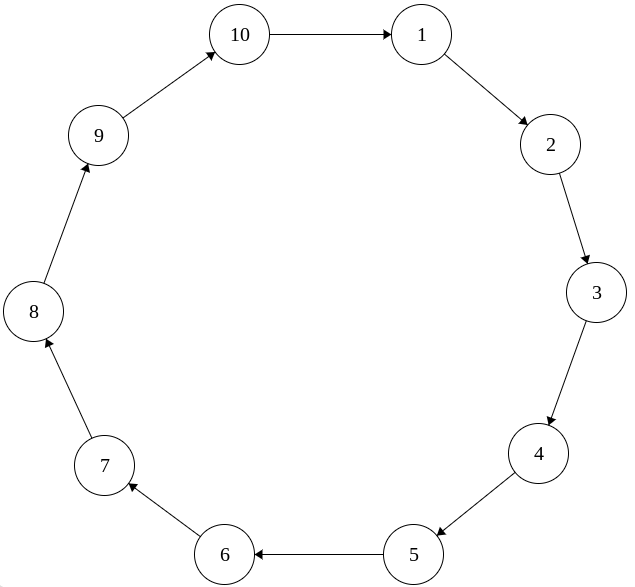
\includegraphics[width=0.6\textwidth]{ForwardCycle}
\end{figure}

Рассмотрим матрицу смежности $A \in M_n(\mathbb{R}_{\max})$ одностороннего цикла на $n$ вершинах.

В силу инвариантности границ относительно домножения на скаляр из $\mathbb{R}$ (замечание \ref{invarianceOfT}), можно рассматривать только тот случай, в котором $\lambda(A) = 0$.
Тогда $\mathcal{G}^c(A) = \mathcal{G}(A)$, $\sigma = n$.
\begin{equation*}
M = (A^n)^* = E^* = E = \begin{pmatrix}
0 & -\infty & ... & -\infty \\
-\infty & 0 & ... & -\infty \\
... & ... & ... & ... \\
-\infty & -\infty & ... & 0
\end{pmatrix} = diag(0, 0, \dots, 0)
\end{equation*}
Значит, $C = R = E$, $S = A$, $B = -\infty$, и для любого неотрицательного $t$ верно $CS^tR[A] = A^t$. Следовательно, $T = T_1 = T_2 = 0$.

\subsection{Двусторонний цикл}
\begin{figure}[h]
% \caption{Односторонний цикл.}
  \centering
    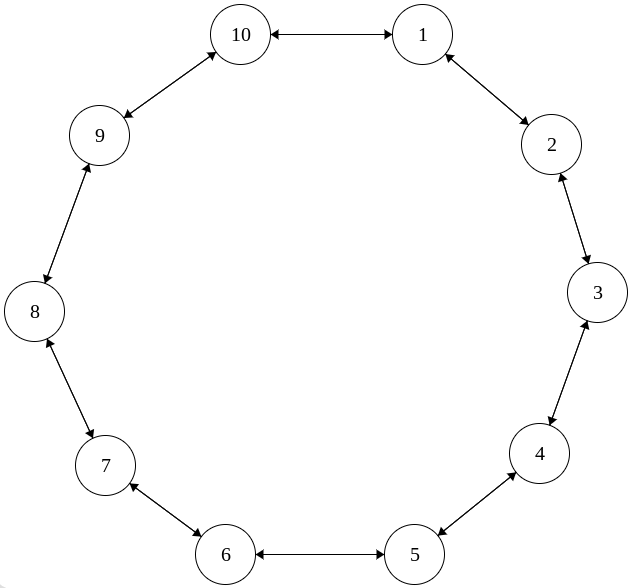
\includegraphics[width=0.6\textwidth]{BidirectionalCycle}
\end{figure}

Рассмотрим матрицу смежности $A \in M_n(\mathbb{R}_{\max})$ двустороннего цикла на $n$ вершинах. Пронумеруем вершины так, чтобы первый цикл состоял из вершин $1, 2, \dots n$(в порядке обхода), а второй --- из $n, n - 1, \dots, 1$ (в порядке обхода). Чтобы избежать кратных рёбер, будем работать с $n \ge 3$.

Будем считать, что $\lambda(A) = 0$. Рассмотрим случай, в котором циклы по часовой стрелке и против часовой стрелки имеют одинаковый средний вес, равный нулю. Значит, критический подграф $\mathcal{G}^c(A)$ совпадает со всем графом $\mathcal{G}(A)$.
\begin{lemma}
Все циклы в таком графе имеют средний вес 0.
\end{lemma}
\begin{proof}[\textbf{Доказательство.}]
Пусть вес пути по часовой стрелке от вершины $i$ до вершины $j$ равен $x$, а против часовой стрелки --- $y$. Эти два пути образуют цикл, значит $x + y \le 0$. Докажем, что $x + y = 0$.

Дополнение к большому циклу по часовой стрелке первого пути весит $-x$, а дополнение к большому циклу против часовой стрелки весит $-y$. Так как можно сначала пойти по дополнению к первому пути, а потом --- по дополнению ко второму пути, эти два дополнения тоже образуют цикл. Значит, $(-x) + (-y) \le 0$. Значит, $x + y \ge 0$.

Следовательно, $x + y = 0$.
\end{proof}
\begin{corollary}
Для фиксированных вершины $i$ и $j$ все пути от $i$ до $j$ весят одинаково.
\end{corollary}

Это верно, так как, в терминах леммы, $x = -y$. Не важно, какой путь выбрать от одной вершины к другой: по или против часовой стрелки --- вес будет одинаковый. Если пройти по большому циклу, то вес не изменится, так как суммарный вес большого цикла равен $0$.

Необходимо рассмотреть 2 случая: когда $n$ нечётно и когда $n$ чётно.

\textbf{n нечетно.} В этом случае цикличность критического графа $\sigma = 1$.

Следовательно, $C = R = M = A^*$, а $S = A$. Заметим, что в матрице $CS^tR[A]$ нет $-\infty$ (так как $CS^tR[A] = A^*A^tA^*$, а в $A^*$ нет $-\infty$). Значит, по следствию из леммы, $CS^tR[A] = A^*$.

Значит, условие $CS^tR[A] = A^t$ верно тогда и только тогда, когда $A^t = A^*$. Поэтому $T = exp(\mathcal{G})$.

\begin{proposition}
Экспонента данного графа равна $n - 1$.
\end{proposition}
\begin{proof}[\textbf{Доказательство.}]
Заметим, что в $A^{n - 2}$ на главной диагонали стоят $-\infty$: $n - 2$ нечётно, поэтому, чтобы вернуться в исходную вершину за $n - 2$ шага, надо сменить чётность --- пройти весь круг, так как остальные циклы имеют чётную длину. Но цикл имеет длину $n$, поэтому его пройти не получится. Значит, $exp(\mathcal{G}) \ge n - 1$.

Покажем, что $A^{n - 1} > -\infty$.

Зафиксируем произвольную вершину $v$ графа. Назовем вершину \textit{четной}, если до нее можно дойти из $v$ за чётное число шагов. Заметим, что тогда все вершины графа четные, так как $n$ нечетно и идти можно как по, так и против часовой стрелки. Наибольшая длина такого пути равна $n - 1$. Значит, $A^{n - 1} > -\infty$.
\end{proof}
\begin{corollary}
$T_2 = 0$, так как $B = -\infty$. $T = T_1 = exp(\mathcal{G}) = n - 1$.
\end{corollary}
\begin{proposition}
Скрамблинг-индекс этого графа равен $\frac{n - 1}{2}$.
\end{proposition}
\begin{proof}[\textbf{Доказательство}]
Пусть $k = k(\mathcal{G})$ --- скрамблинг-индекс данного графа, т. е. для любых двух вершин $u$ и $v$ существуют вершина $w$ такая, что существуют пути из $u$ в $w$ и из $v$ в $w$ длины $k$. В силу неориентированности этого графа это условие равносильно следующему: для любых вершин $u$ и $v$ существует путь из $u$ в $v$ длины $2k$.

Заметим, что для соседних вершин минимальная четная длина пути, соединяющего их, равна $n - 1$, так как $n$ нечетно. Значит, $k \ge \frac{n - 1}{2}$.

Рассмотрим произвольные вершины $i$ и $j$. Пусть два простых пути между ними имеют длину $x$ и $n - x$. Так как $x + (n - x) = n$ --- нечетное число, то среди этих двух путей найдется ровно один с четной длиной. Его длина не превышает $n - 1$ --- наибольшее четное число, не превосходящее $n$. Значит, $k \le \frac{n - 1}{2}$.

Следовательно, $k(\mathcal{G}) = \frac{n - 1}{2}$.
\end{proof}

\textbf{n четно.} В этом случае $\sigma = 2$ и граф не примитивен. $C = R = M = (A^2)^*$, $S = A$.

Так как последовательность матриц $CS^tR$ периодична с периодом $\sigma = 2$ (см. \cite{15WeakCSRExpantion}), то при $t \ge T(A)$ \begin{equation*}
A^t = CS^tR = \begin{cases}
(A^2)^* \text{, если } t \text{ четно.}\\
A \odot (A^2)^*\text{, если } t \text{ нечетно.}\\
\end{cases}
\end{equation*}
В матрице $(A^2)^*$ небесконечные элементы стоят в клетках $(i, j)$, если вершины $i$ и $j$ находятся на четном расстоянии друг от друга. Наибольшее расстояние между вершинами с одинаковой четностью равно $\frac{n}{2}$. Значит, условие при четном $t$ выполняется при $t \ge \frac{n}{2}$, а при прочих $t$ не выполняется.

В матрице $A\odot(A^2)^*$ небесконечные элементы стоят в клетках $(i, j)$, если вершины $i$ и $j$ находятся на нечетном расстоянии друг от друга. Наибольшее расстояние между вершинами с разной четностью равно $\frac{n}{2} - 1$. Значит, условие при четном $t$ выполняется при $t \ge \frac{n}{2} - 1$, а при прочих $t$ --- не выполняется.

Следовательно, $T(A) = \frac{n}{2}$. В силу того, что $B = -\infty$, границы $T_1 = T = \frac{n}{2}$, а $T_2 = 0$, так как $B = -\infty$.

\subsection{Два цикла}
\begin{definition} Назовем ромашкой граф, состоящий из нескольких пересекающихся по одной вершине циклов.
\end{definition}
\label{twoCycles}
Рассмотрим матрицу смежности $A \in M_{2n}(\mathbb{R}_{\max})$ графа-ромашки, состоящего из двух циклов длины $n$ и $n + 1$. Будем называть $n$-циклом цикл длины $n$ и $(n+1)$-циклом --- цикл длины $n + 1$.
\begin{figure}[h]
  \centering
    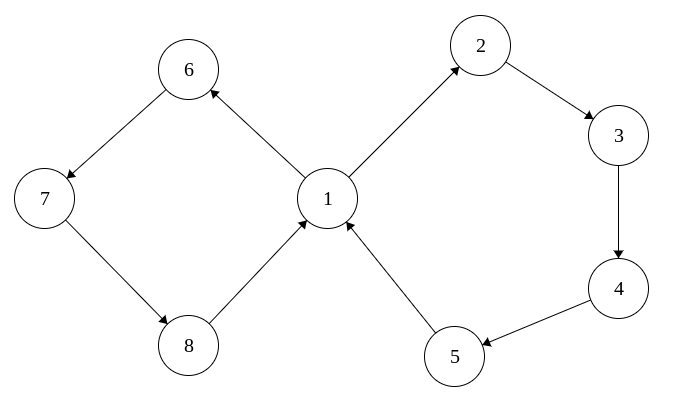
\includegraphics[width=0.6	\textwidth]{2Cycles}
\end{figure}

Будем рассматривать те графы, в которых средний вес каждого цикла равен $0$. Тогда критический подграф совпадает со всем графом: $\mathcal{G}^c(A) = \mathcal{G}(A) = \mathcal{G}$. Его цикличность $\sigma = 1$, значит, $C = R = M = A^*$, а $S = A$.

Следовательно, при $t \ge T(A)$ верно $CS^tR[A] = A^*A^tA^* = A^t$. Так как для произвольных фиксированных вершин любые два пути между ними имеют равные веса, то $T(A) = exp(A)$ (так как в равенстве $A^t = CS^tR[A]$ справа стоит матрица без $-\infty$, а значит и слева должна стоять матрица без $-\infty$).

Это приводит нас к более общему утверждению.

\begin{proposition} \label{onePathProposition}
Если граф $\mathcal{G}(A)$ сильно связен, совпадает со своим критическим подграфом, $\lambda(A) = 0$, его цикличность $\sigma = 1$ и для произвольных двух вершин верно, что все пути между ними имеют одинаковый вес, то $T(A) = T_{1, N}(A) = exp(A)$, а $T_{2,N}(A) = 0$.
\end{proposition}
\begin{proof}[\textbf{Доказательство.}]
Доказательство аналогично предыдущему пункту.

По определению, $M = (A^\sigma)^* = A^*$. Следовательно, $C = R = M = A^*$, а $S = A$.

Значит, при $t \ge T(A)$ верно $CS^tR[A] = A^*A^tA^* = A^t$. В $A^*$ нет $-\infty$, потому что $\mathcal{G}(A)$ сильно связен. Значит, при домножении $A^*$ на матрицу, у которой в каждом столбце есть небесконечный элемент (т.к. граф связен), в результате получится матрица без бесконечностей.

Значит, в левой части равенства нет $-\infty$, поэтому она совпадает с $A^{exp(A)}$. Значит, при $t \ge exp(A)$ выполняется условие на $T(A)$, и $T(A) = exp(A)$.

Так как $B = -\infty$, то $T_{2, N}(A) = 0$, и $T_{1,N}(A) = T(A) = exp(A)$.
\end{proof}
\begin{corollary}
\label{corollaryTandExp}
Утверждение \ref{onePathProposition} верно для многих графов, например, для ромашки из нескольких циклов, для последовательно соединенных циклов. Отметим, что во всех упомянутых графах циклы должны иметь средний вес $0$ и взаимно простую в совокупности длину (граф должен иметь индекс цикличности, равный $1$).
\end{corollary}

\begin{proposition}
Экспонента данного графа равна $n(n+1)$.
\end{proposition}
\begin{proof}[\textbf{Доказательство}]
Докажем, что в $A^{n(n + 1) - 1}$ есть бесконечные элементы. Рассмотрим вершины $i = 2$, $j = n + 1$ и покажем, что в $\mathcal{G}(A)$ не существует пути длины $n(n + 1) - 1$ между $i$ и $j$.

Любой путь из $i$ в $j$, длина которого больше $n - 1$, состоит из трех частей: первая часть --- путь из $i$ в $1$ длины $n$, вторая часть --- $a$ циклов длины $n$, и $b$ циклов длины $n + 1$, идущих в любом порядке. Третья часть --- путь из $1$ в $j$ длины $n$. Таким образом, суммарная длина пути равна $an + b(n + 1) + 2n = (a+2)n + b(n + 1)$.

Покажем, что уравнение \begin{equation}
\label{equation2Cycles}
n(n+1)-1 = (a+2)n + b(n + 1)
\end{equation}
не имеет решений в целых неотрицательных числах относительно $a$ и $b$.

Предположим противное: пусть существуют целые неотрицательные $a, b$, являющиеся решениями \ref{equation2Cycles}. Заметим, что $n(n+1)-1 \equiv -1 \equiv b \pmod{n}$. Значит, $b \ge n - 1$, и\begin{equation*}
n(n+1)-1 = (a+2)n + b(n + 1) \ge (a+2)n + n^2 - 1
\end{equation*}
Следовательно, $n \ge (a + 2)n$, что невозможно в силу неотрицательности $a$.

Значит, уравнение не имеет решений, и в $\mathcal{G}(A)$ нет искомого пути. Следовательно, в $A^{n(n + 1) - 1}$ есть бесконечности и $exp(A) \ge n(n-1)$.

Покажем, что в $A^{n(n + 1)}$ нет бесконечностей. Надо доказать, что для любых вершин $i, j$ существует путь из $i$ в $j$ длины $n(n - 1)$. Пусть расстояние от $i$ до $1$ равно $x$, а расстояние от $1$ до $j$ равно $y$.

Для доказательства утверждения надо показать, что для любых $x, y$ существует решение уравнения $n(n+1) = an + b(n + 1) + x + y$. Заметим, что $x, y \le n$. Пусть $z = x + y$. Рассмотрим \begin{equation*}
(a, b) = \begin{cases}
(z, n - z) & \text{при $0 \le z \le n$} \\
(z - n - 1, 2n - z) & \text{при $n+1 \le z \le 2n$}
\end{cases}
\end{equation*}
Легко проверить, что $a$ и $b$, определенные таким образом, неотрицательны и являются решениями данного уравнения.

Значит, искомый путь всегда найдется, и $exp(A) = n(n + 1)$.
\end{proof}

\begin{proposition}
Скрамблинг-индекс этого графа равен: \begin{equation*}
k(\mathcal{G}) = \begin{cases}
        \frac{n^2 + 2n}{2},     & n \text{ чётно} \\
        \frac{n^2 + 2n - 1}{2}, & n \text{ нечётно}
    \end{cases}
\end{equation*}
\end{proposition}
\begin{proof}[\textbf{Доказательство}]
\begin{definition}
Для $u, v \in V(\mathcal{G})$ введём обозначение:\begin{align*}
k_{u,v}(\mathcal{G}) = \min \{ k \in \mathbb{N} \ | \ \text{существует } w \in V(\mathcal{G}) :\  &\mathcal{W}^k(u \rightarrow w) \neq \varnothing \\
\text{ и } &\mathcal{W}^k(v \rightarrow w) \neq \varnothing\}
\end{align*}
\end{definition}
\begin{lemma}[\cite{scramblingIndex}]
\label{k_uvLemma}
$k(\mathcal{G}) = \max_{u, v \in V(\mathcal{G})} k_{u,v}$.
\end{lemma}

Так как граф в данной задаче фиксирован, обозначим $k_{u,v} = k_{u,v}(\mathcal{G})$.

Найдём формулу для $k_{u,v}$. Для этого надо понять, какой вид имеют оптимальные пути из $u$ в $w$ и из $v$ в $w$.

Заметим, что вершина $w$, определенная для вершин $u$ и $v$, --- это вершина $1$, если $u \neq v$, и вершина $u = v$ иначе. Действительно, если $u = v$, то подходят пути длины ноль и $w = u = v$. Если $u \neq v$ и $w \neq 1$, то у построенных путей есть общий суффикс и их можно укоротить, что противоречит минимальности $k_{u,v}$.

Заметим также, что пути из $u$ в $w$ и из $v$ в $w$ не могут проходить по одному и тому же циклу, иначе оба пути можно было бы укоротить на этот цикл, что противоречило бы с минимальностью $k_{u, v}$.

Рассмотрим случай, когда, без ограничения общности, $u = 1$. Пусть $v$ находится на расстоянии $x$ от вершины $1$ (тогда $0 \le x \le n$).

Путь $u = 1$ состоит из нескольких циклов, а путь $v$ --- это путь длины $x$ от $v$ до $1$, а затем --- несколько циклов.

В силу второго замечания есть $2$ варианта:\begin{enumerate}
\item путь вершины $1$ содержит $(n+1)$-циклы, а вершины $v$ --- $n$-циклы;
\item путь вершины $1$ содержит $n$-циклы, а вершины $v$ --- $(n+1)$-циклы.
\end{enumerate}
Пусть вершина $v$ прошла $a$ циклов, а вершина $1$ --- $b$ циклов ($a, b \ge 0$). Решим для каждого случая уравнение, минимизировав длину пути каждой вершины:
\begin{enumerate}
\item $x + an = b(n + 1)$ --- слева стоит длина пути вершины $v$, а справа --- вершины $1$. Так как мы ищем минимальную длину пути, то необходимо минимизировать левую и правую части.

Заметим, что $b \equiv x \pmod{n}$. Значит, $b \ge x$. Следовательно, решение $a = n - x$, $b = x$ дает минимальную длину путей, которая равна $x(n+1)$.
\item $x + a(n - 1) = bn$. Заметим, что $a \equiv -x \pmod{n}$. Значит, решение $a = n - x$, $b = n - x + 1$ --- оптимальное. Длины путей равны $n(n - x + 1)$.
\end{enumerate}
Таким образом, $k_{1,v} = \min \{x(n+1), n(n - x + 1)\}$.

Рассмотрим случай $u \neq 1$. Пусть расстояние от $u$ до $1$ равно $d_u$, расстояние от $v$ до $1$ равно $d_v$, без ограничения общности $d_u \le d_v$, и $x = d_v - d_u$.

Заметим, что первые $d_u$ рёбер в путях вершин определены однозначно, так как в этом графе есть разветвления только в вершине $1$. После $d_u$ шагов вершина $u$ придет в вершину $1$, и задача сводится к предыдущему случаю.

Значит, $k_{u,v} = d_u + \min \{x(n+1), n(n - x + 1)\}$.

Легко видеть, что максимальное значение $d_u$ равно $n - x$. Оно достигается при $u = ((x + 1)\mod{(n+1)}) + 1$, $v = 2$. Нельзя получить больше, так как вершина $v$ должна оказаться в вершине $1$ через $x + d_u$ шагов, но не раньше. Значит, $x + d_u \le n$ и $d_u \le n - x$.

Следовательно, по лемме \ref{k_uvLemma}:\begin{multline*}
k(\mathcal{G}) = \max_{u, v \in V(\mathcal{G})} d_u + \min \{x(n+1),\; n(n - x + 1)\} =\\= \max_{0 \le x \le n} n - x + \min \{x(n+1),\; n(n - x + 1)\} = 
\max_{0 \le x \le n} \min \{n(x+1),\; n^2 + 2n - x(n+1)\}
\end{multline*}
Требуется найти максимум минимумов двух линейных по $x$ функций. Графики этих функций пересекаются в точке $\hat{x} = \frac{n}{2} + \frac{1}{4} - \frac{1}{4(2n + 1)}$. Значит, максимум 
достигается в одной из целых точек по обе стороны от $\hat{x}$.

Рассмотрим два случая: \begin{itemize}
\item $n$ чётно. Тогда две целые точки по обе стороны от $\hat{x}$ --- это $x_1 = \frac{n}{2}$ и $x_2 = \frac{n + 2}{2}$, при этом в $x_1$ минимумом будет первая функция, а в $x_2$ --- вторая. Значит, \begin{multline*}
k(\mathcal{G}) = \max \{n(x_1+1),\; n^2 + 2n - x_2(n+1) \} =\\= \max \{n(\frac{n}{2}+1),\; n^2 + 2n - \frac{n + 2}{2}(n+1) \} = \frac{n^2+2n}{2}
\end{multline*}
\item $n$ нечётно. Тогда две целые точки по обе стороны от $\hat{x}$ --- это $x_1 = \frac{n-1}{2}$ и $x_2 = \frac{n + 1}{2}$. Значит, \begin{multline*}
k(\mathcal{G}) = \max \{n(x_1+1),\; n^2 + 2n - x_2(n+1) \} =\\= \max \{n(\frac{n-1}{2}+1),\; n^2 + 2n - \frac{n + 1}{2}(n+1) \} = \frac{n^2+2n-1}{2}
\end{multline*}
\end{itemize}
В итоге имеем \begin{equation*}
k(\mathcal{G}) = \begin{cases}
        \frac{n^2 + 2n}{2},     & n \text{ чётно} \\
        \frac{n^2 + 2n - 1}{2}, & n \text{ нечётно}
    \end{cases}
\end{equation*}
\end{proof} 

\subsection{ Ромашка из $p$ циклов длины $k$}
Рассмотрим матрицу смежности $A \in M_{p(k - 1) + 1}(\mathbb{R}_{\max})$ графа-ромашки $\mathcal{G}(A)$, состоящего из $p > 1$ циклов длины $k$ (всего в графе будет $p(k - 1) + 1$ вершин). Будем считать, что вершина, по которой пересекаются все циклы, имеет номер $1$.

Пусть для простоты все ребра в этом графе имеют нулевой вес. Тогда $\mathcal{G}^c = \mathcal{G}(A)$ и $T_2 = 0$, так как $B = -\infty$.
\begin{proposition} Граница $T$, определенная для такого графа-ромашки, равна $k - 1$.
\label{chamomile}
\end{proposition}
\begin{proof}[\textbf{Доказательство.}]
Индекс цикличности этого графа $\sigma = k$. Следовательно, $C = R = M = (A^k)^*$ и $S = A$. По утверждению \ref{entriesInCSR} в ячейке с индексами $i, j$ матрицы $CS^tR$ стоит $0$, если из вершины $i$ можно добраться до вершины $j$ за количество шагов, сравнимое с $t$ по модулю $k$, и $-\infty$ иначе.

Будем говорить, что вершина $v$ имеет класс $i$, если минимальная длина пути между вершинами $1$ и $v$ дает остаток $i$ при делении на $k$. Заметим, что т.к. цикличность графа равна $k$, то длина любого пути из вершины $1$ в $v$ дает остаток $i$ при делении на $k$. Следует упомянуть, что любое ребро ведет из вершины класса $i$ в вершину класса $i + 1 \pmod{k}$.

Покажем, что $T > k - 2$. Рассмотрим вершину $v$ класса $1$ и вершину $u$ класса $k - 1$. Тогда элемент матрицы $CS^{k - 2}R$ с индексами $v, u$ равен $0$. Но в матрице $A^{k - 2}$ элемент с теми же индексами равен $-\infty$, т.к. минимальный путь, соединяющий эти вершины, имеет длину $2k - 2$. Следовательно, $CS^{k - 2}R \neq A^{k - 2}$ и $T \ge k - 1$.

Покажем, что $T = k - 1$. Предположим противное: пусть $T > k - 1$. Рассмотрим $t = T - 1 \ge k - 1$. Заметим, что $CS^{t + k}R = A^{t + k}$, так как $t + k \ge T$.

В матрице $A^{t+k}$ хранится информация о путях длины $t+k$. Но наибольший простой путь имеет длину $2k - 2 < t + k$ --- это путь между вершиной класса $1$ и вершиной класса $k - 1$ из другого цикла. Значит, каждый путь длины $t+k$ можно укоротить на $k$ и получить путь длины $t$ с тем же весом. Значит, $A^{t+k} = A^t$.

По утверждению \ref{periodicity} выполняется равенство $CS^{t + k}R = CS^tR$. Значит, $CS^tR = CS^{t + k}R = A^{t+k} = A^t$. Таким образом, мы получили противоречие с минимальностью $T$, т.к. $t = T - 1$ и $CS^tR = A^t$.

Следовательно, $T = k - 1$.
\end{proof}

\subsection{Ромашка с отрицательными циклами}
\begin{figure}[h]
  \centering
    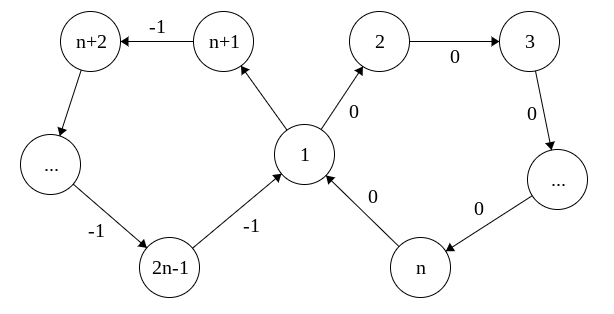
\includegraphics[width=0.7\textwidth]{negativeCycles}
\end{figure}

Рассмотрим матрицу смежности $A \in M_{2n-1}(\mathbb{R}_{\max})$, графа-ромашки, состоящей из двух циклов: цикла длины $n$ с нулевым средним весом (будем называть его нулевым циклом) и цикла длины $n$ с отрицательным средним весом (будем называть его отрицательным циклом). Будем считать, что вершины первого цикла имеют номера от $1$ до $n$ в порядке обхода, а второго --- $1$, $n + 1$, $\dots$, $2n - 1$ в порядке обхода.

\begin{proposition}
$T(A) = T_{1, N}(A) = T_{2, N}(A) = n - 1$.
\label{negativeChalomile}
\end{proposition}
\begin{proof}[\textbf{Доказательство.}]
В этом примере матрица $B$ нетривиальна: она получается из $A$ заменой первых $n$ строк и столбцов на $-\infty$ и кодирует пути в отрицательном цикле. Заметим, что вершина $n$ лежит в критическом подграфе, и, следовательно, инцидентные ей ребра не кодируются матрицей $B$, т.е. $\mathcal{G}(B)$ --- это $n - 1$ последовательная соединенная вершина. Это значит, что $B$ нильпотентна: $B^{n - 1} = -\infty$, так как длиннейший путь в $\mathcal{G}(B)$ имеет длину $n - 2$.

Докажем, что $T_2(A, B) = n - 1$.

В силу нильпотентности $CS^{n - 1}R \ge B^{n - 1} = -\infty$. Значит, $T_2(A, B) \ge n - 1$.

Покажем, что неравенство $CS^tR \ge B^t$ не выполняется при $t = n - 2$.

Рассмотрим вершины $i = n + 1$ и $j = 2n - 1$. Путь, вес которого кодирует ячейка $[B^t]_{ij}$ --- единственная небесконечная ячейка матрицы $B^t$ --- это дуга отрицательного цикла из вершины $i$ в вершину $j$ длины $n - 2$.

Рассмотрим путь, который кодирует ячейка с теми же индексами матрицы $CS^tR$. Он состоит из трех частей: части $C$, части $S^t$, и части $R$. После прохождения части $C$ мы попадем в вершину номер $1$ (так как в матрице $C$ мы делаем произвольное количество шагов длины $n$ и после ее прохождения мы всегда оказываемся в критическом подграфе). Далее в части $S^t$ делаем $n - 2$ шага по критическому подграфу и попадаем в вершину номер $n - 1$. И, наконец, после части $R$ мы оказываемся в вершине $2n - 1$, пройдя еще $n$ шагов.

Посчитаем вес этого пути. Мы целиком прошли нулевой цикл (что не влияет на вес пути, т.к. средний вес ребра в нем равен $0$), целиком прошли отрицательный цикл и еще прошли по простой дуге от $n + 1$-й до $2n - 1$-й вершины. Значит, $[CS^tR + B^t]_{ij} = (\lambda')^{\odot n} \oplus [B^t]_{ij}$, где $\lambda' = \lambda(B) < 0$ --- средний вес отрицательного цикла.

Следовательно, $[CS^tR]_{ij} < [B]_{ij}$, и неверно, что $CS^tR \ge B^t$. Значит, $T_2(A, B) = n - 1$.

Покажем, что $T_1(A, B) = n - 1$. Рассуждения аналогичны доказательству точной оценки для $T(A)$ в утверждении \ref{chamomile}, но с некоторыми изменениями. Назовем путь подходящим, если его вес минимален среди всех путей с концами в тех же вершинах, имеющих ту же длину. Чтобы получить доказательство для графа с отрицательным циклом, надо заменить в доказательстве все слова "путь" на "подходящий путь" (в том графе все пути были подходящими, а в нашем графе --- не все).

Для окончания доказательства надо показать, что любой подходящий путь длины $m > 2n - 2$ можно укоротить на $n$, при этом его вес останется прежним. Действительно, если $m > 2n - 2$, то путь не может быть простым. Значит, в нем есть цикл. Но в подходящем пути не может быть отрицательных циклов, иначе этот цикл можно поменять на нулевой и улучшить ответ. Значит, убрав этот нулевой цикл, можно получить путь между теми же вершинами того же веса, но длины $m - n$. Это завершает доказательство оценки $T_1(A, B)$ для данного графа.
В итоге имеем $T(A) = T_1(A, B) = T_2(A, B) = n - 1$.
\end{proof}

Утверждение \ref{negativeChalomile} верно и для графов-ромашек с большим количеством циклов.
\begin{corollary}
Если $A$ --- матрица смежности графа-ромашки, где каждый цикл имеет длину n и есть хотя бы один нулевой цикл и хотя бы один отрицательный цикл, то $T(A) = T_{1, N}(A) = T_{2, N}(A) = n - 1$.
\end{corollary}

Доказательство этого утверждения аналогично доказательству утверждения \ref{negativeChalomile}.

\subsection{Заключение}
Для некоторых примитивных графов была посчитана их экспонента, скрамблинг-индекс и границы $T$. В каждом примере $k(A(\mathcal{G})) < exp(A) = T(A)$. Более того, в обоих примерах $k(A(\mathcal{G})) \sim \frac{exp(A)}{2}$.

\section{Разные ромашки}
Здесь и далее будем рассматривать графы-ромашки, состоящие из циклов длины, кратной $\sigma$, все рёбра в которых имеют вес $0$. Тогда сразу можно сказать, что у каждой такой ромашки $T_2 = 0$ и $T = T_1$. Для разных таких ромашек будем искать границу $T$.
\begin{definition}
Ромашку, состоящую из циклов длины $a_1\sigma, a_2\sigma, \dots, a_n\sigma$, где числа $a_1, \dots, a_n$ взаимно просты в совокупности, $a_1\le a_2 \le \dots \le a_n$ назовем $(a_1, \dots, a_n; \sigma)$-ромашкой.

Границу $T$, определенную для такой ромашки, будем обозначать через $T(a_1, \dots, a_n; \sigma)$.
\end{definition}

Заметим, что индекс цикличности такой ромашки равен $\sigma$ и всего в ней $N = \sum\limits_{\substack{i=1}}^n a_i\sigma - n + 1$ вершин. Пусть вершина, в которой пересекаются все циклы, имеет номер $1$. Пронумеруем вершины в порядке следующего обхода: начнем в вершине $1$, далее пройдём по первому циклу, затем --- по второму, и так далее до цикла с номером $n$ (не изменяя номер у вершины $1$).

Во всех примерах матрицу смежности рассматриваемого графа будем обозначать через $A \in M_N(\mathbb{R}_{\max})$, а через $C, S, R$ будем обозначать матрицы $C, S, R$, построенные по матрице $A$.

\subsection{Подсчет границы $T$ вручную}
\begin{theorem}
\label{everyKFormula}
$T(a_1, \dots, a_n; \sigma) = (T(a_1, \dots, a_n; 1) + 1)\sigma - 1$.
\end{theorem}
\begin{proof}[\textbf{Доказательство}] 
Обозначим граф, соответствующий $(a_1, \dots, a_n; 1)$-ромашке через $\mathcal{G}$, а граф, соответствующий $(a_1, \dots, a_n; \sigma)$-ромашке --- через $\mathcal{G}_\sigma$. Граф $\mathcal{G}_\sigma$ получается из графа $\mathcal{G}$ разделением каждого ребра на $\sigma$ более мелких рёбер. Вершины $\mathcal{G}_\sigma$, лежащие в одном циклическом классе с вершиной $1$, будем называть начальными. Для краткости будем обозначать $T(a_1, \dots, a_n; 1)$ через $T(1)$, а $T(a_1, \dots, a_n; \sigma)$ --- через $T(\sigma)$.

Покажем, что $T(\sigma) > (T(1) + 1)\sigma - 2$. В $\mathcal{G}$ есть $2$ вершины, между которыми нет пути длины $T(1) - 1$. Значит, в $\mathcal{G}_\sigma$ между соответствующими начальными вершинами нет пути длины $(T(1) - 1)\sigma$. Обозначим эти вершины через $u$ и $v$. Но тогда между вершинами $\hat{u}$ и $\hat{v}$ не будет пути длины $(T(1) - 1)\sigma + 2(\sigma - 1) = (T(1) + 1)\sigma - 2$, где $\hat{u}$ получается, если отойти от $u$ на $\sigma - 1$  шаг вперёд, а $\hat{v}$ --- от вершины $v$ на $\sigma - 1$ шаг назад (обе новые вершины существуют, так как любая вершина в $\mathcal{G}$ лежит в цикле). Значит, $T(\sigma) \ge (T(1) + 1)\sigma - 1$.

Покажем, что $T(\sigma) \ge (T(1) + 1)\sigma - 1$. Для этого нужно доказать, что между любыми двумя вершинами $u$ и $v$ графа $\mathcal{G}_\sigma$ есть путь длины $(T(1) + 1)\sigma - 1$ от $u$ до $v$. Путь длины $(T(1) + 1)\sigma - 1$ от $u$ до $v$ состоит из трех частей: путь от $u$ до ближайшей начальной вершины, путь между начальными вершинами, и путь от ближайшей начальной вершины до $v$. Суммарная длина первой и третьей частей не превосходит $2\sigma - 2$, значит, длина второй части не меньше $(T(1) - 1)\sigma + 1$. Но длина пути между двумя начальными вершинами должна быть кратна $\sigma$, поэтому длина второй части не меньше $T(1)\cdot \sigma$. Но, по определению $T(1)$, между любыми начальными вершинами есть путь длины $T(1)\cdot \sigma$. Значит, $T(\sigma) \ge (T(1) + 1)\sigma - 1$, и утверждение доказано.
\end{proof}
Таким образом, при расчёте границы $T$ для произвольной ромашки достаточно посчитать искомую границу при $\sigma = 1$, а затем получить ответ по формуле \ref{everyKFormula}. 

\begin{remark}
\label{rmrk:expAndT}
При $\sigma = 1$ $(a_1, \dots, a_n; 1)$-ромашка примитивна. Более того, выполняются условия следствия \ref{corollaryTandExp}, и граница $T$ данной ромашки совпадает с экспонентой.
\end{remark}

Введём вспомогательную функцию $P$:
\begin{definition}
Для взаимно простых в совокупности натуральных чисел $a_1 \le \dots \le a_n$ обозначим через $P(a_1, \dots, a_n)$ минимальное целое неотрицательное число, удовлетворяющее следующему свойству: любое $p \ge P(a_1, \dots, a_n)$ выражается в виде линейной комбинации чисел $a_1, \dots, a_n$ с целыми неотрицательными коэффициентами $\lambda_1, \dots, \lambda_n$, то есть $a_1 \lambda_1 + \dots a_n \lambda_n = p$.

Число, выражающееся в виде линейной комбинации чисел $a_1, \dots, a_n$ с целыми неотрицательными коэффициентами, назовём выразимым. Здесь и далее под линейной комбинацией будем понимать линейную комбинацию с целыми неотрицательными коэффициентами.
\end{definition}

\begin{theorem}
\label{thTP}
$T(a_1, \dots, a_n; 1) = P(a_1, \dots, a_n) + 2a_n - 2$.
\end{theorem}
\begin{proof}[\textbf{Доказательство.}]
Предположим, что в $(a_1, \dots, a_n;1)$-ромашке между любыми двумя вершинами существует путь длины $t$. Рассмотрим две произвольные вершины $u$ и $v$. Любой путь длины хотя бы $a_n - 1$ проходит через вершину $1$, и $t \ge a_n - 1$. Поэтому путь длины $t$ от $u$ до $v$ состоит из трёх частей: пути от $u$ до $1$ (обозначим длину этой части через $\hat{u}$), $\lambda_i$ циклов длины $a_i$ для $i = 1\dots n$, и пути от $1$ до $v$ (обозначим длину этой части через $\hat{v})$. Тогда имеет место равенство:
\begin{equation*}
    t = \hat{u} + a_1 \lambda_1 + \dots + a_n \lambda_n + \hat{v} \quad \Longleftrightarrow \quad t - \hat{u} - \hat{v} = a_1 \lambda_1 + \dots + a_n \lambda_n.
\end{equation*}
Сумма $\hat{u} + \hat{v}$ принимает любые значения от $0$ до $2a_n - 2$ (так как $0 \le \hat{u}, \hat{v} \le a_n - 1$). Следовательно, для любого $t - 2a_n + 2 \le p \le t$ должны существовать коэффициенты $\lambda_1, \dots, \lambda_n$, удовлетворяющие уравнению 
\begin{equation}
\label{eqTP}
p = a_1 \lambda_1 + \dots + a_n \lambda_n.
\end{equation}
При $t < P(a_1, \dots, a_n) + 2a_n - 2$ минимальное значение $p$ не превосходит $P(a_1, \dots, a_n) - 1$, и, по определению $P(a_1, \dots, a_n)$, при наименьшем значении $p$ уравнение \ref{eqTP} решений не имеет --- противоречие с наличием пути между $u$ и $v$.

Напротив, при $t \ge P(a_1, \dots, a_n) + 2a_n - 2$ наименьшее значение $p$ не меньше $P(a_1, \dots, a_n)$, и, в силу определения $P(a_1, \dots, a_n)$, коэффициенты $\lambda_i$ найдутся для любого возможного значения $p$.

Значит, $T(a_1, \dots, a_n; 1) = P(a_1, \dots, a_n) + 2a_n - 2$.
\end{proof}

\begin{corollary}[Корректность функции $P$]
Функция $P$ определена корректно: её значение существует для любых возможных аргументов.
\end{corollary}
\begin{proof}[\textbf{Доказательство.}]
Рассмотрим $(a_1, \dots, a_n; 1)$-ромашку. По замечанию \ref{rmrk:expAndT} этот граф примитивен и, следовательно, имеет экспоненту, которая, в свою очередь, совпадает с границей $T$ для данной ромашки. По формуле из теоремы \ref{thTP} имеем $P(a_1, \dots, a_n) = T(a_1, \dots, a_n; 1) - 2a_n + 2$.
\end{proof}

\begin{proposition}[Свойства функции $P$]{\ }
\label{propertiesOfP}
\begin{enumerate}
    \item Если $a_1 = 1$, то $P(1, \dots, a_n) = 0$.
    \item $P(a_1, \dots, a_n) \le P(a_{i_1} , a_{i_2}, \dots, a_{i_k})$, где $1 \le i_1 < i_2 < \dots < i_k \le n$ --- возрастающая последовательность индексов.
    \item $P(a_1, \dots, a_n) = P(b_1, \dots, b_m)$, где набор $b_1, \dots, b_m$ получается из набора $a_1, \dots, a_n$ удалением повторяющихся элементов.
    \item Если $a_j$ делится на $a_i$, то $P(a_1, \dots, a_n) = P(a_1, \dots, a_{j - 1}, a_{j + 1}, \dots, a_n)$.
\end{enumerate}
\end{proposition}
\begin{proof}[\textbf{Доказательство.}]
1) Действительно, если $a_1 = 1$, то любое неотрицательное число $k$ выражается как $1 \cdot k$. Следовательно, $P = 0$.

2) Свойство следует из следующего факта: сумма $a_{i_1} \lambda_{i_1} + \dots + a_{i_k}\lambda_{i_k}$ является частным случаем суммы $a_1 \lambda_1 + \dots + a_n \lambda_n$.

3) При приведении подобных членов в сумме $a_1 \lambda_1 + \dots + a_n \lambda_n$ получается корректная сумма $b_1 \mu_1 + \dots b_m \mu_m$. С другой стороны, сумма $b_1 \mu_1 + \dots b_m \mu_m$ является корректной суммой вида $a_1 \lambda_1 + \dots + a_n \lambda_n$.

4) Очевидно, что любая сумма $a_1 \lambda_1 + \dots + a_{j - 1} \lambda_{j - 1} + a_{j + 1} \lambda_{j + 1} + \dots +a_n \lambda_n$ является суммой вида $a_1 \lambda_1 + \dots + a_n \lambda_n$, где $\lambda_j = 0$. С другой стороны, заменив $a_j$ на $a_i \cdot \frac{a_j}{a_i}$, можно избавиться от слагаемого $a_j \lambda_j$ в сумме $a_1 \lambda_1 + \dots + a_n \lambda_n$, что доказывает утверждение.
\end{proof}

\begin{proposition}
$P(a, b) = (a - 1)(b - 1)$.
\end{proposition}
\begin{proof}[\textbf{Доказательство}]
Покажем, что при $p = ab - a - b \ne ma + nb$ для любых целых неотрицательных $m, n$.

Предположим противное. Тогда: \begin{equation*}
 ab - a - b = am + bn \quad \Longleftrightarrow \quad ab = (m + 1)a + (n + 1) b
\end{equation*}
В силу взаимной простоты $a$ и $b$ получим, что $n + 1 \ \vdots \ a$, и $m + 1 \ \vdots \ b$. Тогда, в силу того, что $m, n \ge 0$, имеем $2$ случая:\begin{align*}
     \begin{cases}
        n + 1 = a\\
        m + 1 = 0
    \end{cases}
    &
    \begin{cases}
        n + 1 = 0\\
        m + 1 = b.
    \end{cases}
\end{align*}
В обоих случаях получаем противоречие. Следовательно, $P(a, b) \ge (a - 1)(b - 1)$.

Теперь покажем, что $P(a, b) \le ab + b - a - 1$. Для любого $p \ge ab - b - a + 1$ решим уравнение: \begin{equation*}
am + bn = p
\end{equation*}
Так как $a$ и $b$ взаимно просты, числа из набора $0, b, 2b, \dots, (a - 1)b$ дают все $a$ остатков по модулю $a$. Значит, существует единственное $0 \le n \le a - 1$, что $bn \equiv p \pmod a$, причём $p - bn \ge 0$, так как 
\begin{equation*}
p - bn \ge ab - b - a + 1 - (a - 1)b = -a + 1 > -a \Longrightarrow p - bn \ge 0.
\end{equation*}
Значит, $m = \frac{p - bn}{a} \ge 0$.

Таким образом, нами были найдены целые $m \ge 0$, $n \ge 0$. Следовательно, $P(a, b) = (a - 1)(b - 1)$.
\end{proof}
\begin{corollary}
$T(a, b; \sigma) = (ab + b - a)\sigma - 1$.
\end{corollary}

\begin{proposition}
$P(2, a, b) = \begin{cases}
P(2, b) = b - 1, &\text{если $a$ чётно,} \\
P(2, a) = a - 1,&\text{иначе.}
\end{cases}$
\end{proposition}
\begin{proof}[\textbf{Доказательство}]
Первый случай следует из свойства 4 утверждения \ref{propertiesOfP}.

Разберём второй случай: $a$ нечётно. Неравенство $P(2, a, b) \le P(2, a)$ следует из свойства $2$ утверждения \ref{propertiesOfP}. Докажем обратное неравенство: необходимо показать, что с помощью слагаемых $2, a, b$ невозможно получить сумму $a - 2$. Действительно, из трёх слагаемых можно использовать только одно: $2$. Но $a - 2$ нечётно --- противоречие. Следовательно, $P(2, a, b) = P(2, a)$.
\end{proof}

\begin{corollary}
$T(2, a, b; \sigma) = \begin{cases}
T(2, b; \sigma) = (3b - 2)\sigma - 1, &\text{если $a$ нечётно,} \\
(2b + a - 2)\sigma - 1, &\text{иначе.}
\end{cases}$
\end{corollary}

\begin{proposition}
$P(3, a, b) = \begin{cases}
P(3, b) = 2(b - 1), \quad \text{если } a \ \vdots \ 3, \\
b - 2, \quad \text{если } a \centernot\vdots 3, a + b \ \vdots \ 3 \text{ и } b < P(3, a) = 2a - 2,\\
P(3, a) = 2(a - 1), \quad \text{иначе.}
\end{cases}$
\end{proposition}
\begin{proof}[\textbf{Доказательство}]
Первый случай следует из свойства 4 утверждения \ref{propertiesOfP}.

Разберём второй случай. Покажем, что $P(3, a, b) \ge b - 2$. Предположим противное. Тогда число $b - 3$ должно выражаться в виде линейной комбинации $2, a$ и $b$:
\begin{equation*}
b - 3 = 3 \lambda_1 + a \lambda_2 + b \lambda_3
\end{equation*}
Тогда $\lambda_3 = 0$ и $\lambda_2 \le 1$. При $\lambda_2 = 0$ имеем $b = 3\lambda_1 + 3 \ \vdots \ 3$. При $\lambda_2 = 1$ имеем $b - a = 3\lambda_1 + 3 \ \vdots \ 3$. В обоих случаях $a \ \vdots \ 3$, так как $a + b \ \vdots \ 3$, что противоречит условию второго случая. Следовательно, $P(3, a, b) \ge b - 2$.


Докажем обратное неравенство: для любого $p \ge b - 2$ решим уравнение:
\begin{equation*}
p = 3 \lambda_1 + a \lambda_2 + b \lambda_3
\end{equation*}
Так как в правой части есть слагаемое $3 \lambda_1$, то достаточно решить уравнение для $p = b - 2$, $p = b - 1$ и $p = b$ --- тогда линейные комбинации для больших $p$ получатся увеличением $\lambda_1$.
\begin{itemize}
\item $p = b - 2$. Если $b \equiv 2 \pmod 3$, то $\lambda_1 = \frac{b - 2}{3}, \lambda_2 = \lambda_3 = 0$.

Если $b \equiv 1 \pmod 3$, то $a \equiv 2 \pmod 3$, $b - 2 = (b - a - 2) + a$ и $\lambda_1 = \frac{b - a - 2}{3}, \lambda_2 = 1, \lambda_3 = 0$.
\item $p = b - 1$. Если $b \equiv 1 \pmod 3$, то $\lambda_1 = \frac{b - 1}{3}, \lambda_2 = \lambda_3 = 0$.

Если $b \equiv 2 \pmod 3$, то $a \equiv 1 \pmod 3$, $b - 2 = (b - a - 1) + a$ и $\lambda_1 = \frac{b - a - 1}{3}, \lambda_2 = 1, \lambda_3 = 0$.
\item $p = b$. Тогда $\lambda_1 = \lambda_2 = 0, \lambda_3 = 1$.
\end{itemize}

Таким образом, $P(3, a, b) = b - 2$.

Перейдём к третьему случаю: если $b \ge P(3, a)$, то наличие слагаемого $b \lambda_3$ не повлияет на значение функции $P$: если некое $p$ выражается в виде линейной комбинации с участием $b$, то $p \ge P(3, a)$ и, следовательно, выражается и без участия $b$. Следовательно, $P(3, a, b) = P(a, b)$.

Рассмотрим последний случай: $a \centernot\vdots 3,\ a + b \ \centernot\vdots \ 3, \ b < P(3, a)$. Неравенство $P(3, a, b) \ge P(a, b)$ следует из свойства $2$ утверждения \ref{propertiesOfP}. Докажем обратное неравенство. Для этого покажем, что следующее уравнение не имеет решений:
\begin{equation*}
    2a - 3 = 3 \lambda_1 + a \lambda_2 + b \lambda_3
\end{equation*}
Заметим, что $\lambda_3 = 0$, так как $b < 2a - a$. Также, $\lambda_2 \le 1$. Тогда $(2 - \lambda_2)a = 3\lambda_1 + 3 \ \vdots \ 3$ --- противоречие с $a \centernot\vdots 3$. Значит, $P(3, a, b) = P(a, b)$.
\end{proof}

\begin{corollary}
$T(3, a, b; 1) = \begin{cases}
T(3, b; 1) = 4b - 4, &\text{если } a \ \vdots \ 3, \\
3b - 4, &\text{если } a \centernot\vdots 3, a + b \ \vdots \ 3 \text{ и } m < 2a - 2,\\
2a + 2b - 4, &\text{иначе.}
\end{cases}$
\end{corollary}

\subsection{Алгоритм вычисления функции $P$}
\begin{lemma}
\label{algorithm:lemma1}
Число $p$ выразимо тогда и только тогда, когда $p = 0$ или выразимо хотя бы одно из чисел $p - a_1, \dots, p - a_n$.
\end{lemma}
\begin{proof}[\textbf{Доказательство}]
Докажем необходимость: пусть некоторое $p > 0$ выразимо: $p = a_1 \lambda_1 + \dots + a_n \lambda_n$. Тогда хотя бы одно из чисел $\lambda_1, \dots, \lambda_n$ положительно: пусть $\lambda_i > 0$. Тогда выразимо число $p - a_i = a_1 \lambda_1 + \dots + a_i \cdot(\lambda_i - 1) + \cdot + a_n \lambda_n$.

Докажем достаточность. Очевидно, что $p = 0$ выразимо. Если $p > 0$ и выразимо число $p - a_i$, то выразимо и $p$: достаточно увеличить $\lambda_i$ в линейной комбинации для $p - a_i$ на единицу.
\end{proof}

\begin{lemma}
\label{algorithm:lemma2}
$P(a_1, \dots, a_n) = p$ тогда и только тогда, когда $p - 1$ не выразимо, а числа $p, p + 1, \dots, p + a_1 - 1$ выразимы.
\end{lemma}
\begin{proof}[\textbf{Доказательство}]
Необходимость следует из определения функции $P$.

Докажем достаточность: пусть числа $p, p + 1, \dots, p + a_1 - 1$ выразимы. Тогда выразимо любое число, не меньшее $p$: для любого $x \ge p$ существует единственное число $k$ такое, что $p \le x - k \cdot a_1 \le p + a_1 - 1$, то есть $x - k \cdot a_1$ выразимо. Увеличив коэффициент $\lambda_1$ в линейной комбинации для $x - k \cdot a_1$ на $k$, получим линейную комбинацию для $x$. Значит, $P(a_1, \dots, a_n) \le p$.

Так как $p - 1$ невыразимо, имеем $P(a_1, \dots, a_n) \ge p$. Следовательно, $P(a_1, \dots, a_n) = p$.
\end{proof}

Приведём алгоритм, позволяющий вычислять функцию $P$. Для этого предположим, что некая функция $ANS$ оценивает сверху функцию $P$: $P(a_1, \dots, a_n) \le ANS(a_1, \dots, a_n)$.
\begin{algorithm}
\label{algorithm}
\begin{enumerate}
    \item Создадим массив $dp$ длины $ANS + a_1$, заполненный нулями. В $dp[p]$ будет лежать $0$, если $p$ невыразимо, и $1$ --- иначе.
    \item Поместим в $dp[0]$ значение $1$ --- $0$ выразим всегда.
    \item Проверим каждое значение $p$ от $1$ до $ANS + a_1$ на выразимость. Для этого переберём числа $p - a_i$ для $1 \le i \le n$. Если хотя бы одно из значений $dp[p - a_i]$ равно $1$, то $p$ выразимо и $dp[p] = 1$, иначе $dp[p] = 0$.
    \item Когда мы впервые обнаружим $a_1$ последовательно лежащих единиц (то есть\\  $dp[p - a_1 + 1] = dp[p - a_1 + 2] = \dots = dp[p])$, то ответом будет $p - a_i + 1$. 
\end{enumerate}
\end{algorithm}

\begin{proposition}
Алгоритм \ref{algorithm} работает корректно; время его работы равно $O(n \cdot (ANS + a_1))$.
\end{proposition}
\begin{proof}[\textbf{Доказательство}]
Докажем корректность. Шаг 3 верен по лемме \ref{algorithm:lemma1}. Шаг 4 --- по лемме \ref{algorithm:lemma2}.

Докажем асимптотику. Всего будет проверено ровно $P(a_1, \cdot, a_n) + 1$ значений $p$, что не превосходит $ANS + a_1$, и каждая проверка будет работать за $O(n)$. Итоговая асимптотика --- $O(n \cdot (ANS + a_1))$.
\end{proof}

\subsection{Верхние оценки функции $P$}
Оценим сверху значение функции $P$. Это поможет и в оценке сверху границы $T$ для ромашек, и для уточнения времени работы алгоритма \ref{algorithm}.

\begin{proposition}
$P(a_1, \dots, a_n) \le Wi(N) - 2a_n + 2$, где $N = \sum\limits_{\substack{i=1}}^n a_i - n + 1$ --- количество вершин в $(a_1, \dots, a_n; 1)$-ромашке.
\end{proposition}
\begin{proof}[\textbf{Доказательство}]
По замечанию \ref{rmrk:expAndT} граница $T$ данной ромашки совпадает с её экспонентой, которая по теореме \ref{tropicalWielandtTh} оценивается сверху числом Виландта от количества вершин $Wi(N) = N^2 - 2N + 2$.

Значит, по теореме \ref{thTP}, $P(a_1, \dots, a_n) + 2a_n - 2 = T(a_1, \dots, a_n; 1) \le Wi(N)$. Следовательно, $P(a_1, \dots, a_n) \le Wi(N) - 2a_n + 2 = N^2 - 2N + 2 - 2a_n + 2$.
\end{proof}

\begin{corollary}
Асимптотика алгоритма \ref{algorithm} --- $O(n \cdot N^2)$.
\end{corollary}
\begin{proof}[\textbf{Доказательство}]
При подстановке $Wi(N) + 2a_2 - 2$ вместо функции $ANS$ имеем асимптотику $O(n \cdot (N^2 - 2N + 2 - 2a_n + 2 + a_1)) = O(n \cdot N^2)$ (так как $N = \sum\limits_{\substack{i=1}}^n a_i - n + 1$).
\end{proof}

\begin{proposition}
\label{P:LC}
$P(a_1, \dots, a_n) \le P(b_1, \dots, b_m)$, где каждое из чисел $b_j$ выражается в виде линейной комбинации чисел $a_i$.
\end{proposition}
\begin{proof}[\textbf{Доказательство}]
Рассмотрим линейную комбинацию чисел $b_j$: $b_1\mu_1 + \dots + b_m \mu_m$. При раскрытии скобок и приведении подобных членов получим сумму вида $a_1 \lambda_1 + \dots + a_n \lambda_n$, что доказывает утверждение.
\end{proof}

\begin{corollary}
$P(a_1, \dots, a_n) \le P(a_1, a_2 + \dots + a_n) = (a_1 - 1)(N + n - 1 - a_1)$.
\end{corollary}
\begin{proof}[\textbf{Доказательство}]
Заметим, что числа $a_1$ и $a_2 + \dots + a_n$ взаимно просты. Далее утверждение следует по утверждению \ref{P:LC}.
\end{proof}

\begin{corollary}
Асимптотика алгоритма \ref{algorithm} --- $O(n \cdot a_1 \cdot (N + n - a_1))$.
\end{corollary}
\begin{proof}[\textbf{Доказательство}]
Подставив $(a_1 - 1)(N + n - 1 - a_1)$ вместо функции $ANS$, имеем асимптотику $O(n \cdot ((a_1 - 1) \cdot (N + n - 1 - a_1) + a_1)) = O(n \cdot a_1 \cdot (N + n - a_1))$.
\end{proof}

\section{Границы $T$ и скрамблинг-индекс}
\begin{definition}
Рассмотрим произвольную матрицу $X \in M_{n+m}(\mathbb{R}_{\max})$ размера $n + m$. Назовем $n$-$m$-декомпозицией матрицы $X$ следующие четыре матрицы:\begin{align*}
X_{11} \in M_{n \times n}(\mathbb{R}_{\max}) & \quad X_{12} \in M_{n \times m}(\mathbb{R}_{\max}) \\
X_{21} \in M_{m \times n}(\mathbb{R}_{\max}) & \quad X_{22} \in M_{m \times m}(\mathbb{R}_{\max}),
\end{align*}
такие, что \begin{equation*}
X = \begin{pmatrix}
X_{11} & X_{12} \\
X_{21} & X_{22}
\end{pmatrix}.
\end{equation*}
\end{definition}

Рассмотрим граф $\mathcal{G}$ на $n + m$ вершинах, матрицей смежности $A \in M_{n+m}(\mathbb{R}_{\max})$ и с положительным скрамблинг-индесом $k(\mathcal{G})$. По критерию положительности скрамблинг-индекса (\ref{theorem:ScramblingIndexCriteria}) в $\mathcal{G}$ существует примитивный достижимый подграф $\mathcal{G}_2$.  Обозначим через $\mathcal{G}_1$ индуцированный подграф исходного графа $\mathcal{G}$, порожденный множеством вершин $V(\mathcal{G}) \textbackslash V(\mathcal{G}_2)$.

Для удобства перенумеруем вершины: пусть в графе $\mathcal{G}_1$ лежат вершины с номерами от $1$ до $n$, а в $\mathcal{G}_2$ --- от $n + 1$ до $n + m$. Тогда в $n$-$m$-декомпозиции матрицы $A$ в матрице $A_{ij}$ лежит информация о ребрах из $\mathcal{G}_i$ в $\mathcal{G}_j$.

Будем рассматривать те графы, для которых $\mathcal{G}^c = \mathcal{G}_2$ и $\lambda(A) = 0$. Так как граф $\mathcal{G}_2$ примитивен, его цикличность равна $1$. Значит, $M = A^*$.

Рассмотрим $n$-$m$-декомпозицию матрицы $M$:
\begin{equation*}
M = \begin{pmatrix}
M_{11} & M_{12}\\
M_{21} & M_{22}
\end{pmatrix}.
\end{equation*}

\begin{proposition}
Матрица $M_{ij}$ имеет вид:
\begin{equation*}
M_{ij} = (A^*)_{ij} = \bigoplus_{t = 0}^{n + m - 1}\bigoplus_{\sigma}\bigodot_{k = 0}^{t - 1} A_{\sigma(k), \sigma(k + 1)},
\end{equation*}
где $i, j \in \{1, 2\}$, $\sigma \in \{1, 2\}^{t + 1}$, причем $\sigma(0) = i$, $\sigma(t) = j$.
\end{proposition}
\begin{proof}[\textbf{Доказательство.}]
Матрицы $C, R, S, B$ имеют вид:
\begin{equation*}
C = \begin{pmatrix}
-\infty & M_{12}\\
-\infty & M_{22}
\end{pmatrix}, 
R = \begin{pmatrix}
-\infty & -\infty \\
M_{21} & M_{22}
\end{pmatrix}, 
S = \begin{pmatrix}
-\infty & -\infty \\
-\infty & A_{22}
\end{pmatrix},
B = \begin{pmatrix}
A_{11} & -\infty \\
-\infty & -\infty
\end{pmatrix}.
\end{equation*}
Для $t \ge T(A)$ верно следующее равенство:
\begin{multline*}
A^t = CS^tR = \begin{pmatrix}
-\infty & M_{12}\\
-\infty & M_{22}
\end{pmatrix} \odot \begin{pmatrix}
-\infty & -\infty \\
-\infty & A_{22}
\end{pmatrix}^t \odot \begin{pmatrix}
-\infty & -\infty \\
M_{21} & M_{22}
\end{pmatrix} = \\
= \begin{pmatrix}
	M_{12}A_{22}^tM_{21} & M_{12}A_{22}^tM_{22} \\
	M_{22}A_{22}^tM_{21} & M_{22}A_{22}^tM_{22}
\end{pmatrix},
\end{multline*}
для $t \ge T_1(A, B)$ --- следующее:
\begin{equation*}
A^t = CS^tR \oplus B^t = \begin{pmatrix}
	M_{12}A_{22}^tM_{21} \oplus A_{11}^t & M_{12}A_{22}^tM_{22} \\
	M_{22}A_{22}^tM_{21} & M_{22}A_{22}^tM_{22}
\end{pmatrix},
\end{equation*}
и для $t \ge T_2(A, B)$ --- следующее неравенство:
\begin{equation*}
\begin{pmatrix}
	M_{12}A_{22}^tM_{21} & M_{12}A_{22}^tM_{22} \\
	M_{22}A_{22}^tM_{21} & M_{22}A_{22}^tM_{22}
\end{pmatrix} \ge \begin{pmatrix}
A_{11}^t & -\infty \\
-\infty & -\infty
\end{pmatrix},
\end{equation*} т.е., что равносильно, $M_{12}A_{22}^tM_{21} \ge A_{11}^t$.

Выразим $A^t$: 
\begin{equation*}
(A^t)_{ij} = \bigoplus_{\sigma}\bigodot_{k = 0}^{t - 1} A_{\sigma(k), \sigma(k + 1)},
\end{equation*}
где $i, j \in \{1, 2\}$, $\sigma \in \{1, 2\}^{t + 1}$, причем $\sigma(0) = i, \sigma(t) = j$. Здесь и далее считаем, что $\sigma(k)$ --- это $k$-й элемент кортежа $\sigma$, нумерация в котором идет с нуля.

Рассмотрим путь из произвольной вершины подграфа $\mathcal{G}_i$ в произвольную вершину подграфа $\mathcal{G}_j$. Каждое ребро этого пути либо лежит внутри соответствующего подграфа, либо соединяет текущий подграф с другим. Переберем все возможные варианты расположения ребер в пути: если $\sigma(k-1) = \sigma(k)$, то $k$-е ребро пути лежит в графе $\mathcal{G}_{\sigma(k-1)}$. Иначе --- ведёт из $\mathcal{G}_{\sigma(k-1)}$ в $\mathcal{G}_{\sigma(k)}$. По всем таким вариантам возьмем максимум --- это и будет оптимальным весом пути.

Зафиксируем $i, j \in \{1, 2\}$. Тогда матрица $M_{ij}$ выражается следующим образом:
\begin{equation*}
M_{ij} = (A^*)_{ij} = \bigoplus_{t = 0}^{n + m - 1}\bigoplus_{\sigma}\bigodot_{k = 0}^{t - 1} A_{\sigma(k), \sigma(k + 1)},
\end{equation*}
где $\sigma \in \{1, 2\}^{t + 1}$, причем $\sigma(0) = i$, $\sigma(t) = j$.
\end{proof}
\section{Обозначения}
\begin{enumerate}
    \item ${\mathbb{R}_{\geq0}}$ --- множество неотрицательных вещественных чисел.
    
    \item $\mathbb{R}_{\max}, \mathbb{R}_{\min}$ --- тропические полукольца.
   
    \item $\mathbb{B} = \{\textbf{0,1}\}$ --- множество с сложением, аналогичным дизъюнкции, и умножением, аналогичным конъюнкции.
    
    \item $M_{n \times m}(\mathbb{F})$ --- множество матриц $n \times m$ с элементами из $\mathbb{F}$.
    
    $M_n(\mathbb{F})$ --- множество квадратных матриц $n \times n$ с элементами из $\mathbb{F}$.
    
    \item $[M]_{ij}$ --- элемент матрицы $M$ с индексами $i$ и $j$.
    
    \item ${\mathcal{G}(V,E)}$ --- граф со множеством вершин $V$ и множеством ребер $E$.
    
    \item $Wi(n) = (n - 1)^2 + 1$ --- число Виландта.
    
    \item $DM(\hat{g}, n) =  \hat{g}(n - 2) + n$, где $\hat{g} = \hat{g}(\mathcal{G}^c(A))$ --- число Далмаджа-Мендельсона.
    
\begin{comment}    
    \item $\mathbb{PT}$ --- множество прямоугольных тропических матриц без бесконечных строк и столбцов.
\end{comment}
    
    \item $\sigma_\mathcal{G}$ --- индекс цикличности графа $G$.
    
    \item $k(\mathcal{G})$ --- скрамблинг индекс графа $G$.
    
    \item $g(\mathcal{G})$ --- обхват графа $\mathcal{G}$, т.е. длина наименьшего цикла в $\mathcal{G}$.
    
    \item $\hat{g}(\mathcal{G})$ --- максимальный обхват среди всех компонент сильной связности графа $\mathcal{G}$.
    
    \item $exp(\mathcal{G})$ --- экспонента графа (а значит, и его матрицы смежности).
    
    \item $\lambda(A)$ --- максимальный средний вес цикла в графе $\mathcal{G}(A)$.
    
    \item $\mathcal{G}^c$ --- критический подграф графа $\mathcal{G}$.
    
    \item $A^*$ --- звезда Клини матрицы $A$.
    
    \item $\mathcal{W}(i \rightarrow j)$ --- множество путей из вершины $i$ в вершину $j$.
    
    $\mathcal{W}^t(i \rightarrow j)$ --- множество путей из вершины $i$ в вершину $j$ длины $t$.
    
    $\mathcal{W}^{t, l}(i \rightarrow j)$ --- множество путей из вершины $i$ в вершину $j$ длины $t$ по модулю $l$.
    
    \item $\mathcal{W}(i \xrightarrow{\mathcal{G}} j)$, $\mathcal{W}^t(i \xrightarrow{\mathcal{G}} j)$, $\mathcal{W}^{t, l}(i \xrightarrow{\mathcal{G}} j)$ --- аналогично предыдущему пункту, но с дополнительным условием на путь: он должен проходить хотя бы через одну вершину из $\mathcal{G}$.
    
    \item $T(A), T_1(A, B), T_2(A, B)$ --- границы, определенные в подразделе \ref{subsection:CSR}.
\end{enumerate}

\begin{thebibliography}{9}
\bibitem{ImreSimon}
Imre Simon
\textit{\href{http://www.numdam.org/item?id=ITA_1994__28_3-4_277_0}{On semigroups of matrices over the tropical semiring}}
Theoretical Informaties and Applications (Tome 28 (1994) no. 3-4, pp. 277-294)

\bibitem{glanceOnTropicalLA}
Semere Tsehaye Tesfay.
\textit{A Glance at Tropical Operations and Tropical Linear Algebra}
Eastern Illinois University, 2015.

\bibitem{tropicalMath}
David Speyer, Bernd Sturmfels.
\textit{Tropical Mathematics}
Mathematics Magazine, vol. 82, №3, June 2009.

\bibitem{Volchenko}
Ю.М. Волченко
\textit{\href{http://yura.volchenko.com/Science/Max-plus.pdf}{Max-plus алгебра и ее применение}}, декабрь 2017

\bibitem{wielandt}
Hans Schneider.
\textit{Wielandt’s proof of the exponent inequality for
primitive nonnegative matrices}
Department of Mathematics, University of Wisconsin at Madison, 2002.

\bibitem{chainable}
Ю.А. Альпин, И.В. Башкин.
\textit{Неотрицательные цепные матрицы}
Казанский федеральный университет, 2020.

\bibitem{cyclicity}
Alexander Guterman, Elena Kreines, and Carsten Thomassen.
\textit{Linear transformations of tropical matrices
preserving the cyclicity index}
Special Matrices Volume 9, 2021.

\bibitem{scramblingIndex}
A. E. Guterman, A. M. Maksaev
\textit{Upper bounds on scrambling index for non-primitive digraphs}
Linear and Multilinear Algebra, 2019

\bibitem{bounds}
Arthur Kennedy-Cochran-Patrick, Glenn Merlet, Thomas Nowak, Sergei Sergeev.
\textit{New bounds on the periodicity transient of the powers of a tropical matrix: Using cyclicity and factor rank}
Linear Algebra and its Applications, 2020

\bibitem{15WeakCSRExpantion}
Glenn Merlet, Thomas Nowak, Sergei Sergeev.
\\\textit{https://www.sciencedirect.com/science/article/pii/S0024379514004777}

\bibitem{21CSRExpansionsOfMatrixPowersInMaxAlgebra}
Sergei Sergeev, Hans Schneider.
\textit{CSR expansions of matrix powers in max algebra} Transactions of the American Mathematical Society, December 2009

\bibitem{Brualdi}
Brualdi RA, Ryser HJ. \textit{Combinatorial matrix theory.} Cambridge: Cambridge University Press;
1991. (Encyclopedia of mathematics and its applications; 39).
\end{thebibliography}

\end{document}